% notes on coupling coefficients for SU(2)
\documentclass{article}[10pt]
\usepackage{fullpage}
\usepackage{amsmath}
\usepackage{graphicx}

%%%%%%%%%%%%%%%%%%%%%%%%%%%%%%%%%%%%%%%%%%%%%%%%%%%%%%%%%%%%%%%%%%%%%%%%%%%%%%%%
%%                                                                            %%
%%             MACRO FILE for the PhD thesis of Ian Peter McCulloch           %%
%%                                                                            %%
%%                  (Last modified: Sunday 16th March, 1997)                  %%
%%                                                                            %%
%%%%%%%%%%%%%%%%%%%%%%%%%%%%%%%%%%%%%%%%%%%%%%%%%%%%%%%%%%%%%%%%%%%%%%%%%%%%%%%% 


%%%%%%%%%%%%%%%%%%%%%%%%%%%%%%%%%%%%%%%%%%%%%%%%%%%%%%%%%%%%%%%%%%%%%%%%%%%%%%%%
%%       NEW COMMANDS AND SHORTHAND NOTATIONS                                 %%
%%%%%%%%%%%%%%%%%%%%%%%%%%%%%%%%%%%%%%%%%%%%%%%%%%%%%%%%%%%%%%%%%%%%%%%%%%%%%%%%


%%%%%%%%%%%%%%%%%%%%%%%%%%%%%%%%%%%%%%%%%%%%%%%%%%%%%%%%%%%%%%%%%%%%%%%%%%%%%%%%
%%                                                                            %%
%%       Definition of some useful Commands                                   %%
%%                                                                            %%
%%       \militarytime   :  24hr clock time                                   %%
%%       \beq            :  \begin{equation}                                  %%
%%       \eeq            :  \end{equation}                                    %%
%%       \bea            :  \begin{eqnarray}                                  %%
%%       \eea            :  \end{eqnarray}                                    %%
%%       \beqstar        :  \begin{displaymath}                               %%
%%       \eeqstar        :  \end{displaymath}                                 %%
%%       \beastar        :  \begin{eqnarray*}                                 %%
%%       \eeastar        :  \end{eqnarray*}                                   %%
%%       \vektor         :  bold math                                         %%
%%       \smvektor       :  small bold math                                   %%
%%       \refeq{#1}      :  refer to an equation as Eq. (\ref{#1})            %%
%%       \refsec{#1}      :  refer to a section as section \ref{#1}           %%
%%       \reffig{#1}     :  refer to a figure as Fig. \ref{#1}                %%
%%       \sreffig{#1}    :  refer to a figure as Fig. \ref{#1}  (start of sentence) %%
%%                             (designed for the start of a sentence)         %%
%%       \drawbox        :  draws a box at (#1,#2) of size #3 x#4             %%
%%       \drawdmrg       :  draws schematic DMRG blocks at (#1,#2) of         %%
%%                          widths #3 (left block) and #4 (right block)       %%
%%                                                                            %%

   \newcount\hour
   \newcount\minute
   \newtoks\amorpm
   \hour=\time\divide\hour by60
   \minute=\time{\multiply\hour by60 \global\advance\minute by-\hour}
   \edef\militarytime{\number\hour:\ifnum\minute<10 0\fi\number\minute}

   \newcommand{\beq}{\begin{equation}}
   \newcommand{\eeq}{\end{equation}}
   \newcommand{\bea}{\begin{eqnarray}}
   \newcommand{\eea}{\end{eqnarray}}
   \newcommand{\beqstar}{\begin{displaymath}}
   \newcommand{\eeqstar}{\end{displaymath}}
   \newcommand{\beastar}{\begin{eqnarray*}}
   \newcommand{\eeastar}{\end{eqnarray*}}
   \newcommand{\vektor}[1]{\mbox{\boldmath $#1$}}
   \newcommand{\smvektor}[1]{\mbox{\boldmath \scriptsize $#1$}}
   \newcommand{\refeq}[1]{Eq.\ (\ref{#1})}
   \newcommand{\refsec}[1]{section \ref{#1}}
   \newcommand{\reffig}[1]{Fig.\ \ref{#1}}
   \newcommand{\sreffig}[1]{Fig.\ \ref{#1}}

   \newcount\x \newcount\xx \newcount\y \newcount\yy

\def\drawbox#1#2#3#4{
\x=#1 \y=#2 \xx = #1 \advance \xx by #3 \yy = #2 \advance \yy by #4
\put(\x,\y){\line(1,0){#3}}
\put(\x,\yy){\line(1,0){#3}}
\put(\x,\y){\line(0,1){#4}}
\put(\xx,\y){\line(0,1){#4}}
}

\def\drawdmrg#1#2#3#4{
\drawbox{#1}{#2}{#3}{2}
\x=#1
\y=#2
\xx=#1 \advance \xx by 1 \advance \xx by #3
\yy=#2 \advance \yy by 1
\put(\xx,\yy){\circle*{0.8}}
\advance \xx by 2
\put(\xx,\yy){\circle*{0.8}}
\advance \xx by 1
\drawbox{\xx}{\y}{#4}{2}
}

%%                                                                            %%
%%%%%%%%%%%%%%%%%%%%%%%%%%%%%%%%%%%%%%%%%%%%%%%%%%%%%%%%%%%%%%%%%%%%%%%%%%%%%%%%


%%%%%%%%%%%%%%%%%%%%%%%%%%%%%%%%%%%%%%%%%%%%%%%%%%%%%%%%%%%%%%%%%%%%%%%%%%%%%%%%
%%                                                                            %%
%%       Definition of some common Text Shorthands                            %%
%%                                                                            %%
%%       \ie          :  i.e.     id est                     (that is)        %%
%%       \eg          :  e.g.     exempli gratia             (for example)    %%
%%       \etc         :  etc.     et cetera                  (and so on)      %%
%%       \etal        :  et al.   et alii/aliae/alia/alius   (and others)     %%
%%       \cf          :  cf.      confer                     (compare)        %%
%%       \cetpar      :  ceteris paribus               (all else being equal) %%
%%       \apriori     :  a priori                      (from cause to effect) %%
%%       \perse       :  per se                              ( by itself)     %%
%%       \viceversa   :  vice versa                           ( in reverse)   %%
%%       \primafacie  :  prima facie   (sufficient unless or until disproved) %%
%%                                                                            %%

   \newcommand{\ie}{\mbox{\it i.e. \/}}
   \newcommand{\eg}{\mbox{\it e.g. \/}}
   \newcommand{\etc}{\mbox{\it etc. \/}}
   \newcommand{\etal}{\mbox{\it et al. \/}}
   \newcommand{\cf}{\mbox{\it cf. \/}}
   \newcommand{\cetpar}{\mbox{\it ceteris paribis \/}}
   \newcommand{\apriori}{\mbox{\it a priori \/}}
   \newcommand{\perse}{\mbox{\it per se \/}}
   \newcommand{\viceversa}{\mbox{\it vice versa \/}}
   \newcommand{\primafacie}{\mbox{\it prima facie \/}}

%%                                                                            %%
%%%%%%%%%%%%%%%%%%%%%%%%%%%%%%%%%%%%%%%%%%%%%%%%%%%%%%%%%%%%%%%%%%%%%%%%%%%%%%%%


%%%%%%%%%%%%%%%%%%%%%%%%%%%%%%%%%%%%%%%%%%%%%%%%%%%%%%%%%%%%%%%%%%%%%%%%%%%%%%%%
%%                                                                            %%
%%       Definition of some common Mathematical Symbols and Notation          %%
%%                                                                            %%
%%       \rat=Q       :  The set of Rational Numbers                          %%
%%       \nat=N       :  The set of Natural Numbers                           %%
%%       \integer=Z   :  The set of Integers  (I have a replacement!)         %%
%%       \reals=R     :  The set of Real Numbers                              %%
%%       \field=K     :                                                       %%
%%       \complex=C   :  The set of Complex Numbers                           %%
%%       \domain=D    :                                                       %%
%%                                                                            %%
%%       \smallfrac{#1}{#2}       :  Produces a small fraction                %%
%%       \bmath{#1}               :  Produces bold math characters            %%
%%       \bmaths{#1}              :  Produces scriptsize bold math characters %%
%%                                :  (especially for lower case greek letters)%%
%%       \bigsum                  :  Produces a big summation sign            %%
%%       \bigint                  :  Produces a big integral sign             %%
%%       \bigprod                  :  Produces a big product sign             %%
%%                                                                            %%
%%       \chem{#1}                :  chemical formula. Roman math.            %%
%%       \tr       \Tr            :  Trace of a matrix                        %%
%%       \real     \imag          :  Real and Imaginary parts                 %%
%%       \plus     \minus         :  + and - with smaller spaces              %%
%%       \te  \tz  \td  \tv       :  The 4 standard theta functions (1,2,3,4) %%
%%   \p \q \qs  \ELL \ELLs \ELLt  :  The elliptic nome and quantum group par. %%
%%       \ket{#1}                 :  Dirac notation | #1 >                    %%
%%       \bra{#1}                 :  Dirac notation < #1 |                    %%
%%       \rket{#1}                :  reduced ket  || #1 >                     %%
%%       \rbra{#1}                :  reduced bra < #1 ||                      %%
%%       \mpket{#1}               :  Dirac notation | #1 >_{MP}               %%
%%       \braket{#2}              :  < #1 | #2 >                              %%
%%       \rbraket{#2}             :  < #1 || #2 >                             %%
%%       \bigbraket{#3}           :  < #1 | #2 | #3 >                         %%
%%       \mpbigbraket{#3}         :  < #1 | #2 | #3 >_{MP}                    %%
%%       \rbigbraket{#3}          :  < #1 || #2 || #3 >                       %%
%%       \com{#2}                 :  [#1,#2]                                  %%
%%       \anticom{#2}             :  \{#1,#2\}                                %%
%%       \itensor                 :  \vektor{#1}^{[#2]}                       %%
%%       \itensordag                 :  \vektor{#1}^{\dagger[#2]}             %%
%%       \citensor                 :  \vektor{\bar{#1}}^{[#2]}                %%
%%       \itensorcomp             :  \hbox{{#1}^{[#2]}_{#3}}                  %%
%%       \itensors                :  \vektor{#1}^{[#2]}_{#3}                  %%
%%       \itensorss               :  \vektor{#1}^{[#2]#3}_{#4}                %%
%%       \smitensor               :  \smvektor{#1}^{[#2]}                     %%
%%       \itensorcoupling}        :  \left( #1 \bmath{\times}#2\right)^{[#3]} %%
%%       \JRKKY                   :  J_{RKKY}                                 %%
%%       \rmsub{#1}               :  roman scriptsize                         %%
%%                                                                            %%

   \makeatletter

   \newcommand{\nat}{{\rm I \mkern-2.5mu \nonscript\mkern-.5mu I \mkern-5.5mu 
                      N}} 
%   \newcommand{\integer}{{\setbox0\hbox{\m@th$\fam\sffam Z$}
%                          \setbox1\hbox{\rm\kern.05\wd0 \rlap{\vrule 
%                          height.93\ht0 depth-.75\ht0 width.056\wd0 }%
%                          \kern-.13\wd0 \copy0 \kern-.6\wd0 \copy0 
%                          \kern-.1\wd0 \llap{\vrule height.25\ht0 depth\z@ 
%                          width.056\wd0}% 
%                          \kern.05\wd0} \mathchoice{\copy1}{\copy1}{\mit 
%                          Z\mkern-8mu Z}{\mit Z\mkern-7.5mu Z} }} 
   \newcommand{\integer}{\:\mbox{\sf Z} \hspace{-0.82em} \mbox{\sf Z}\,}
   \def\@@insvline#1#2{{\setbox0\hbox{\m@th$#1\rm I$} \rlap{\m@th$#1 \mkern5mu 
                        \vrule height.92\ht0 depth-.05\ht0 width.09\ht0 $} 
                        {\rm #2} }} 
   \newcommand{\rat}{\mathpalette\@@insvline{Q}}
   \newcommand{\reals}{{\rm I \mkern-2.5mu \nonscript\mkern-.5mu R}}
   \newcommand{\complex}{\mathpalette\@@insvline{C}} 
   \newcommand{\field}{{\rm I \mkern-2.5mu \nonscript\mkern-.5mu K}} 
   \newcommand{\domain}{{\rm I \mkern-2.5mu \nonscript\mkern-.5mu D}} 
   \newcommand{\smallfrac}[2]{\mbox{\small $\frac{#1}{#2}$}}
   \newcommand{\bmath}[1]{\mbox{\boldmath{$#1$}}}
   \newcommand{\bmaths}[1]{\mbox{\boldmath{\scriptsize $#1$}}}

   \font\largesignfont=cmex10 scaled \magstep2
   \newcommand{\bigint}[2]{\hbox{$\textfont3=\largesignfont\displaystyle
               \int_{#1}^{#2}$}}
   \newcommand{\bigsum}[2]{\hbox{$\textfont3=\largesignfont\displaystyle
               \,\sum_{#1}^{#2}\,$}}
   \newcommand{\bigprod}[2]{\hbox{$\textfont3=\largesignfont\displaystyle
               \,\prod_{#1}^{#2}\,$}}
   
   \newcommand{\tr}{\mathop{\rm tr}}
   \newcommand{\Tr}{\mathop{\rm Tr}}
   \newcommand{\real}{\mathop{\it {\Re}e}}
   \newcommand{\imag}{\mathop{\it {\Im}m}}
   \newcommand{\plus}{\mathop{\!+\!}}
   \newcommand{\minus}{\mathop{\!-\!}}
   \newcommand{\te}{\vartheta_1}
   \newcommand{\tz}{\vartheta_2}
   \newcommand{\td}{\vartheta_3}
   \newcommand{\tv}{\vartheta_4}
   \newcommand{\p}{\mbox{p}}
   \newcommand{\q}{\mbox{q}}
   \newcommand{\qs}{\mbox{\scriptsize q}}
   \newcommand{\ELL}{\mathrm{L}}
   \newcommand{\ELLs}{\mathrm{\scriptscriptstyle L}}
   \newcommand{\ELLt}{\mbox{\tiny L}}
   \newcommand\vpint{{\rm -}\kern -1.1em\int_{-\infty}^\infty}

   \newcommand{\ket}[1]{\hbox{$\mid \! {#1} \rangle$}}
   \newcommand{\bra}[1]{\langle #1 |}

   \newcommand{\rket}[1]{\| #1 \rangle}
   \newcommand{\rbra}[1]{\langle #1 \|}

   \newcommand{\mpket}[1]{| #1 \rangle_{\scriptstyle MP}}
   \newcommand{\mpbigbraket}[3]{\langle \, #1 \, | \, #2 \, | \, #3 \, \rangle_{\scriptstyle MP}}
   \newcommand{\mpbraket}[2]{\langle \, #1 \, | \, #2 \, \rangle_{\scriptstyle MP}}

   \newcommand{\braket}[2]{\langle #1 | #2 \rangle}
   \newcommand{\bigbraket}[3]{\langle \, #1 \, | \, #2 \, | \, #3 \, \rangle}

   \newcommand{\rbraket}[2]{\langle #1 \| #2 \rangle}
   \newcommand{\rbigbraket}[3]{\langle \, #1 \, \| \, #2 \, \| \, #3 \, \rangle}

   \newcommand{\com}[2]{{\big[} #1 \, , \, #2 {\big]}}
   \newcommand{\anticom}[2]{{\big\{} #1 \, , \, #2 {\big\}}}

   \newcommand{\gcom}[3]{\left[ #1 \, , \, #2 \right]^{[#3]}}
   \newcommand{\ganticom}[3]{\left\{ #1 \, , \, #2 \right\}^{[#3]}}

   \newcommand{\theorem}[1]{{\it #1}}

   \newcommand{\definition}[2]{{\bf Definition} \quad {\it #1} \\ {#2}}

   \newcommand{\itensor}[2]{\hbox{$\vektor{#1}^{[#2]}$}}
   \newcommand{\citensor}[2]{\hbox{$\vektor{\bar{#1}}^{[#2]}$}}
   \newcommand{\itensorcomp}[3]{\hbox{${#1}^{[#2]}_{#3}$}}
   \newcommand{\itensors}[3]{\hbox{$\vektor{#1}^{[#2]}_{#3}$}}
   \newcommand{\itensorss}[4]{\hbox{$\vektor{#1}^{[#2]#3}_{#4}$}}
   \newcommand{\smitensor}[2]{\hbox{$\smvektor{#1}^{\scriptscriptstyle [#2]}$}}

   \newcommand{\itensordag}[2]{\hbox{$\vektor{#1}^{\dagger[#2]}$}}
   \newcommand{\itensordags}[3]{\hbox{$\vektor{#1}^{\dagger[#2]}_{#3}$}}


   \newcommand{\itensorcoupling}[3]{\hbox{${\big[} #1 \bmath{\times} #2 {\big]}$}^{[#3]}}

   \newcommand{\itensoroutercoupling}[3]{\hbox{${\big[} #1 \bmath{\otimes} #2 {\big]}$}^{[#3]}}

   \newcommand{\lsim}{\;{\lower4pt\hbox{$\stackrel  {\displaystyle <} \sim$}}\;}
   \newcommand{\gsim}{\;{\lower4pt\hbox{$\stackrel  {\displaystyle >} \sim$}}\;}

   \newcommand{\rmsub}[1]{\mbox{\scriptsize #1}}

   \newcommand{\JRKKY}{J_{\mbox{\scriptsize RKKY}}}

   \newcommand{\chem}[1]{\hbox{$\rm #1$}}

   \makeatother

%%                                                                            %%
%%%%%%%%%%%%%%%%%%%%%%%%%%%%%%%%%%%%%%%%%%%%%%%%%%%%%%%%%%%%%%%%%%%%%%%%%%%%%%%%


%%%%%%%%%%%%%%%%%%%%%%%%%%%%%%%%%%%%%%%%%%%%%%%%%%%%%%%%%%%%%%%%%%%%%%%%%%%%%%%%
%%                                                                            %%
%%      Definition of some useful  Shorthands                                 %%
%%                                                                            %%
%%                            {1}{2}{3}                                       %%
%%      \qcg              :  C                                                %%
%%                            {4}{5}{6}                                       %%
%%                                                                            %%
%%                            ( {1}{2}{3} )                                   %%
%%      \qsixj            :   <           >                                   %%
%%                            ( {4}{5}{6} ){7}                                %%
%%                                                                            %%
%%      \qthreej         :    ( {1}{2}{3} )                                   %%
%%                            ( {4}{5}{6} )                                   %%

   \newcommand{\qcg}[6]{ \mbox{$C {}^{#1}_{#4} {}^{#2}_{#5} {}^{#3}_{#6}$} }

   \newcommand{\gencg}[7]{ \mbox{$\left( {}^{#1}_{#2} {}^{#3}_{#4} \vert 
                {}^{#5}_{#6} {}^{,#7} \right)$} }

   \newcommand{\gencginv}[7]{ \mbox{$\left( {}^{#3,}_{} {}^{#1}_{#2} \vert 
        {}^{#4}_{#5} {}^{#6}_{#7} \right)$} }

   \newcommand{\qracah}[6]{ W \left( {#1},{#2},{#3},{#4} ; {#5},{#6} \right) }

   \newcommand{\qsixj}[6]{\mbox{$\left\{ \begin{array}{ccc} \!{#1}\! &
                                \!{#2}\! & \!{#3}\! \\ \!{#4}\! & \!{#5}\! &
                                \!{#6}\! \end{array} \right\}$}}

   \newcommand{\qthreej}[6]{\mbox{$\left( \begin{array}{ccc} \!{#1}\! &
                                \!{#2}\! & \!{#3}\! \\ \!{#4}\! & \!{#5}\! &
                                \!{#6}\! \end{array} \right)$}}

   \newcommand{\qsixjx}[7]{\mbox{$\left\{ \begin{array}{ccc} \!{#1}\! &
                                \!{#2}\! & \!{#3}\! \\ \!{#4}\! & \!{#5}\! &
                                \!{#6}\! \end{array} \right\}_{\!\!\mbox{\scriptsize 
                                #7}}$}}

   \newcommand{\qninej}[9]{\mbox{$\left\{ \begin{array}{ccc} \!{#1}\! &
                                \!{#2}\! & \!{#3}\! \\ \!{#4}\! & \!{#5}\! &
                                \!{#6}\! \\ \!{#7}\! & \!{#8}\! & \!{#9}\! 
                                \end{array} \right\}$}}

   \newcommand{\qninejsq}[9]{\mbox{$\left[ \begin{array}{ccc} \!{#1}\! &
                                \!{#2}\! & \!{#3}\! \\ \!{#4}\! & \!{#5}\! &
                                \!{#6}\! \\ \!{#7}\! & \!{#8}\! & \!{#9}\! 
                                \end{array} \right]$}}

%%                                                                            %%
%%%%%%%%%%%%%%%%%%%%%%%%%%%%%%%%%%%%%%%%%%%%%%%%%%%%%%%%%%%%%%%%%%%%%%%%%%%%%%%%


%%%%%%%%%%%%%%%%%%%%%%%%%%%%%%%%%%%%%%%%%%%%%%%%%%%%%%%%%%%%%%%%%%%%%%%%%%%%%%%%
%%                                                                            %%
%%      Definition of some useful S-matrix and Lattice Stat. Mech. Pictures   %%
%%                                                                            %%
%%      \picsmatrix{a}{b}{c}{d}{theta1}{theta2}                               %%
%%      \picupcoupling{a}{b}{c}                                               %%
%%      \picdowncoupling{a}{b}{c}                                             %%
%%      \picleftfactorisation                                                 %%
%%      \picrightfactorisation                                                %%
%%      \picleftbootstrap                                                     %%
%%      \picrightbootstrap                                                    %%
%%      \picboltzmannweight{a}{b}{u}{v}{k}                                    %%
%%      \pictransfermatrix{a}{b}{u}{v}{k}                                     %%
%%      \piclattice                                                           %%
%%      \pickinkprojmap                                                       %%
%%      \pickinkscatt                                                         %%
%%      \picstheta                                                            %%
%%      \pictwopart                                                           %%
%%                                                                            %%

   \newcommand{\picsmatrix}[6]{\setlength{\unitlength}{4mm}
                  \rule[-3.7\unitlength]{0mm}{6\unitlength}
                  \hspace{4\unitlength} \begin{picture}(4,3)(0,0)
                  {\thicklines
                  \put(-3.0,-2.5){\line(1,1){5}} \put(-3.0,2.5){\line(1,-1){5}}
                  }
                  \put(-2.5,-0.2){\makebox(0,0)[c]{\mbox{$#1$}}}
                  \put(1.5,-0.2){\makebox(0,0)[c]{\mbox{$#2$}}}
                  \put(-0.5,-2.0){\makebox(0,0)[c]{\mbox{$#3$}}}
                  \put(-0.5,1.8){\makebox(0,0)[c]{\mbox{$#4$}}}
                  \put(-3.2,-3.2){\makebox(0,0)[c]{\mbox{$#5$}}}
                  \put(2.4,-3.2){\makebox(0,0)[c]{\mbox{$#6$}}}
                  \end{picture}}
   \newcommand{\picupcoupling}[3]{\setlength{\unitlength}{3mm}
                  \rule[-3.7\unitlength]{0mm}{6\unitlength}
                  \hspace{4\unitlength} \begin{picture}(4,3)(0,0)
                  {\thicklines
                  \put(-0.5,0){\line(-1,-1){2.5}}
                  \put(-0.5,0){\line(1,-1){2.5}}
                  \put(-0.5,0){\line(0,1){2.8}}
                  }
                  \put(-2.2,0.6){\makebox(0,0)[c]{\mbox{$#1$}}}
                  \put(1.2,0.6){\makebox(0,0)[c]{\mbox{$#2$}}}
                  \put(-0.5,-2.0){\makebox(0,0)[c]{\mbox{$#3$}}}
                  \end{picture}}
   \newcommand{\picdowncoupling}[3]{\setlength{\unitlength}{3mm}
                  \rule[-3.7\unitlength]{0mm}{6\unitlength}
                  \hspace{4\unitlength} \begin{picture}(4,3)(0,0)
                  {\thicklines
                  \put(-0.5,0){\line(-1,1){2.5}}
                  \put(-0.5,0){\line(1,1){2.5}}
                  \put(-0.5,0){\line(0,-1){2.8}}
                  }
                  \put(-2.2,-0.6){\makebox(0,0)[c]{\mbox{$#1$}}}
                  \put(1.2,-0.6){\makebox(0,0)[c]{\mbox{$#2$}}}
                  \put(-0.5,2.0){\makebox(0,0)[c]{\mbox{$#3$}}}
                  \end{picture}}
   \newcommand{\picleftfactorisation}{\setlength{\unitlength}{3mm}
                  \rule[-9\unitlength]{0mm}{6\unitlength} \hspace{6\unitlength}
                  \begin{picture}(8,8)(0,0) 
                  {\thicklines 
                  \put(-1.5,-7.5){\line(0,1){15}}
                  \put(-5.5,6.0){\line(3,-2){12.2}}
                  \put(-5.5,-6.0){\line(3,2){12.2}}
                  }
                  \put(-3.4,-0.1){\makebox(0,0)[c]{\mbox{$\alpha$}}}
                  \put(-3.0,-6.2){\makebox(0,0)[c]{\mbox{$\beta$}}}
                  \put(2.0,-4.2){\makebox(0,0)[c]{\mbox{$\gamma$}}}
                  \put(5.8,0.0){\makebox(0,0)[c]{\mbox{$\delta$}}}
                  \put(2.0,3.6){\makebox(0,0)[c]{\mbox{$\epsilon$}}}
                  \put(-3.0,6.0){\makebox(0,0)[c]{\mbox{$\eta$}}}
                  \put(0.2,-0.2){\makebox(0,0)[c]{\mbox{$\mu$}}}
                  \put(-5.8,-6.8){\makebox(0,0)[c]{\mbox{$\theta_{1}$}}}
                  \put(-1.4,-8.4){\makebox(0,0)[c]{\mbox{$\theta_{2}$}}}
                  \put(7.4,-2.6){\makebox(0,0)[c]{\mbox{$\theta_{3}$}}}
                  \end{picture}
                  \hspace{2\unitlength}}
   \newcommand{\picrightfactorisation}{\setlength{\unitlength}{3mm}
                  \rule[-9\unitlength]{0mm}{6\unitlength}
                  \hspace{10\unitlength} \begin{picture}(8,8)(0,0)
                  {\thicklines
                  \put(1.5,-7.5){\line(0,1){15}}
                  \put(5.5,6.0){\line(-3,-2){12.2}}
                  \put(5.5,-6.0){\line(-3,2){12.2}}
                  }
                  \put(-5.6,-0.1){\makebox(0,0)[c]{\mbox{$\alpha$}}}
                  \put(2.9,-6.1){\makebox(0,0)[c]{\mbox{$\gamma$}}}
                  \put(-2.2,-4.2){\makebox(0,0)[c]{\mbox{$\beta$}}}
                  \put(3.4,0.0){\makebox(0,0)[c]{\mbox{$\delta$}}}
                  \put(-2.2,3.6){\makebox(0,0)[c]{\mbox{$\eta$}}}
                  \put(3.1,6.0){\makebox(0,0)[c]{\mbox{$\epsilon$}}}
                  \put(-0.3,-0.2){\makebox(0,0)[c]{\mbox{$\mu$}}}
                  \put(6.2,-6.6){\makebox(0,0)[c]{\mbox{$\theta_{3}$}}}
                  \put(1.6,-8.4){\makebox(0,0)[c]{\mbox{$\theta_{2}$}}}
                  \put(-7.0,-3.0){\makebox(0,0)[c]{\mbox{$\theta_{1}$}}}
                  \end{picture}}
   \newcommand{\picleftbootstrap}{\setlength{\unitlength}{3mm}
                  \rule[-9\unitlength]{0mm}{6\unitlength}
                  \hspace{6\unitlength} \begin{picture}(8,8)(0,0)
                  {\thicklines
                  \put(-1.0,-2.5){\line(-1,-1){3.5}}
                  \put(-1.0,-2.5){\line(1,-4){1.0}}
                  \put(-1.0,-2.5){\line(2,5){2.0}}
                  \put(1.0,2.5){\line(1,1){3.5}}
                  \put(1.0,2.5){\line(-1,4){1.18}}
                  \put(-5.0,2.0){\line(2,-1){10.0}}
                  }
                  \put(-3.4,-1.8){\makebox(0,0)[c]{\mbox{$\alpha$}}}
                  \put(-2.0,-5.6){\makebox(0,0)[c]{\mbox{$\beta$}}}
                  \put(1.6,-3.8){\makebox(0,0)[c]{\mbox{$\gamma$}}}
                  \put(3.0,0.8){\makebox(0,0)[c]{\mbox{$\delta$}}}
                  \put(1.8,4.8){\makebox(0,0)[c]{\mbox{$\epsilon$}}}
                  \put(-1.8,2.8){\makebox(0,0)[c]{\mbox{$\eta$}}}
                  \put(-4.8,-6.8){\makebox(0,0)[c]{\mbox{$\theta_{1}$}}}
                  \put(0.4,-7.4){\makebox(0,0)[c]{\mbox{$\theta_{2}$}}}
                  \put(5.8,-3.6){\makebox(0,0)[c]{\mbox{$\theta_{3}$}}}
                  \end{picture}
                  \hspace{2\unitlength}}
   \newcommand{\picrightbootstrap}{\setlength{\unitlength}{3mm}
                  \rule[-9\unitlength]{0mm}{6\unitlength}
                  \hspace{10\unitlength} \begin{picture}(8,8)(0,0)
                  {\thicklines
                  \put(-1.0,-2.5){\line(-1,-1){3.5}}
                  \put(-1.0,-2.5){\line(1,-4){1.0}}
                  \put(-1.0,-2.5){\line(2,5){1.0}}
                  \put(0.0,0.0){\line(1,1){6.0}}
                  \put(0.0,0.0){\line(-1,4){1.8}}
                  \put(-5.5,6.0){\line(2,-1){12.0}}
                  }
                  \put(-3.0,0.4){\makebox(0,0)[c]{\mbox{$\alpha$}}}
                  \put(-2.0,-5.6){\makebox(0,0)[c]{\mbox{$\beta$}}}
                  \put(2.4,-2.0){\makebox(0,0)[c]{\mbox{$\gamma$}}}
                  \put(5.4,2.8){\makebox(0,0)[c]{\mbox{$\delta$}}}
                  \put(1.4,4.8){\makebox(0,0)[c]{\mbox{$\epsilon$}}}
                  \put(-2.8,6.0){\makebox(0,0)[c]{\mbox{$\eta$}}}
                  \put(0.6,1.8){\makebox(0,0)[c]{\mbox{$\mu$}}}
                  \put(7.2,-0.6){\makebox(0,0)[c]{\mbox{$\theta_{3}$}}}
                  \put(0.4,-7.4){\makebox(0,0)[c]{\mbox{$\theta_{2}$}}}
                  \put(-4.8,-6.8){\makebox(0,0)[c]{\mbox{$\theta_{1}$}}}
                  \end{picture}}
   \newcommand{\picboltzmannweight}[5]{\setlength{\unitlength}{4mm}
                  \hspace{2\unitlength} \rule[-3.7\unitlength]{0mm}{
                  6.2\unitlength} \begin{picture}(6,3)(0,-0.3)
                  {\thicklines
                  \put(2.5,-2.5){\line(0,1){5}} \put(5,0){\line(-1,0){5}}
                  }
                  \put(2.6,-3.4){\makebox(0,0)[b]{\mbox{$#4_{#5}$}}}
                  \put(-0.5,0){\makebox(0,0)[r]{\mbox{$#3$}}}
                  \put(1.4,0.8){\makebox(0,0)[b]{\mbox{$#2_{#5}$}}}
                  \put(4.1,0.8){\makebox(0,0)[b]{\mbox{$#2_{#5+1}$}}}
                  \put(1.4,-1.4){\makebox(0,0)[b]{\mbox{$#1_{#5}$}}}
                  \put(4.1,-1.4){\makebox(0,0)[b]{\mbox{$#1_{#5+1}$}}}
                  \end{picture}}
   \newcommand{\pictransfermatrix}[5]{\setlength{\unitlength}{4mm}
                  \hspace{2\unitlength} \rule[-3.7\unitlength]{0mm}{
                  6.2\unitlength} \begin{picture}(17,3)(0,-0.3) 
                  {\thicklines
                  \put(2.5,-2.5){\line(0,1){5}} \put(6,-2.5){\line(0,1){5}}
                  \put(8.5,0){\line(-1,0){8.5}} \put(11.5,0){\line(1,0){5}}
                  \put(14,-2.5){\line(0,1){5}} 
                  }
                  \put(9.4,0){\makebox(0,0)[l]{\mbox{$\ldots$}}} 
                  \put(-0.5,0){\makebox(0,0)[r]{\mbox{$#3$}}}
                  \put(2.7,-3.4){\makebox(0,0)[b]{\mbox{$#4_{1}$}}}
                  \put(6.2,-3.4){\makebox(0,0)[b]{\mbox{$#4_{2}$}}}
                  \put(14.3,-3.4){\makebox(0,0)[b]{\mbox{$#4_{#5}$}}}
                  \put(1.4,0.8){\makebox(0,0)[b]{\mbox{$#2_{1}$}}}
                  \put(4.3,0.8){\makebox(0,0)[b]{\mbox{$#2_{2}$}}}
                  \put(15.4,0.8){\makebox(0,0)[b]{\mbox{$#2_{1}$}}}
                  \put(7.4,0.8){\makebox(0,0)[b]{\mbox{$#2_{3}$}}}
                  \put(12.9,0.8){\makebox(0,0)[b]{\mbox{$#2_{#5}$}}}
                  \put(1.4,-1.4){\makebox(0,0)[b]{\mbox{$#1_{1}$}}}
                  \put(4.3,-1.4){\makebox(0,0)[b]{\mbox{$#1_{2}$}}}
                  \put(15.4,-1.4){\makebox(0,0)[b]{\mbox{$#1_{1}$}}}
                  \put(7.4,-1.4){\makebox(0,0)[b]{\mbox{$#1_{3}$}}}
                  \put(12.9,-1.4){\makebox(0,0)[b]{\mbox{$#1_{#5}$}}}
                  \end{picture}}

   \newcommand{\piclattice}{\setlength{\unitlength}{12mm}
                  \begin{picture}(10,9.5)(0,-0.5)
                  {\thicklines
                  \multiput(1.0,0.0)(1,0){3}{\line(0,1){3.5}}
                  \multiput(1.0,5.5)(1,0){3}{\line(0,1){2.5}}
                  \multiput(8.0,0.0)(1,0){2}{\line(0,1){3.5}}
                  \multiput(8.0,5.5)(1,0){2}{\line(0,1){2.5}}
                  \multiput(0.0,1.0)(0,1){3}{\line(1,0){3.5}}
                  \multiput(7.5,1.0)(0,1){3}{\line(1,0){2.5}}
                  \multiput(0.0,6.0)(0,1){2}{\line(1,0){3.5}}
                  \multiput(7.5,6.0)(0,1){2}{\line(1,0){2.5}}
                  \qbezier[30](3.5,1.0)(5.5,1.0)(7.5,1.0)
                  \qbezier[30](3.5,2.0)(5.5,2.0)(7.5,2.0)
                  \qbezier[30](3.5,3.0)(5.5,3.0)(7.5,3.0)
                  \qbezier[30](3.5,6.0)(5.5,6.0)(7.5,6.0)
                  \qbezier[30](3.5,7.0)(5.5,7.0)(7.5,7.0)
                  \qbezier[15](0.985,3.5)(0.985,4.5)(0.985,5.5)
                  \qbezier[15](1.99,3.5)(1.99,4.5)(1.99,5.5)
                  \qbezier[15](2.99,3.5)(2.99,4.5)(2.99,5.5)
                  \qbezier[15](7.985,3.5)(7.985,4.5)(7.985,5.5)
                  \qbezier[15](8.985,3.5)(8.985,4.5)(8.985,5.5)
                  \qbezier[34](3.625,3.625)(5.5,4.5)(7.375,5.375)
                  }
                  {\thinlines
                  \multiput(0.5,0.5)(0.267,0){12}{\line(1,0){0.1}}
                  \multiput(7.5,0.5)(0.272,0){8}{\line(1,0){0.1}}
                  \multiput(0.5,7.5)(0.267,0){12}{\line(1,0){0.1}}
                  \multiput(7.5,7.5)(0.27,0){8}{\line(1,0){0.1}}
                  \multiput(0.5,0.5)(0,0.26){12}{\line(0,1){0.18}}
                  \multiput(9.5,0.5)(0,0.26){12}{\line(0,1){0.18}}
                  \multiput(0.5,5.5)(0,0.26){8}{\line(0,1){0.18}}
                  \multiput(9.5,5.5)(0,0.26){8}{\line(0,1){0.18}}
                  \qbezier[30](3.5,0.5)(5.5,0.5)(7.5,0.5)
                  \qbezier[30](3.5,7.5)(5.5,7.5)(7.5,7.5)
                  \qbezier[15](0.49,3.5)(0.49,4.5)(0.49,5.5)
                  \qbezier[15](9.495,3.5)(9.495,4.5)(9.495,5.5)
                  }
                  \put(-0.5,1.0){\makebox(0,0)[c]{\mbox{$u_{1}$}}}
                  \put(-0.5,2.0){\makebox(0,0)[c]{\mbox{$u_{2}$}}}
                  \put(-0.5,3.0){\makebox(0,0)[c]{\mbox{$u_{3}$}}}
                  \put(-0.5,6.0){\makebox(0,0)[c]{\mbox{$u_{M-1}$}}}
                  \put(-0.5,7.0){\makebox(0,0)[c]{\mbox{$u_{M}$}}}
                  \put(1.05,-0.5){\makebox(0,0)[c]{\mbox{$v_{1}$}}}
                  \put(2.1,-0.5){\makebox(0,0)[c]{\mbox{$v_{2}$}}}
                  \put(3.1,-0.5){\makebox(0,0)[c]{\mbox{$v_{3}$}}}
                  \put(8.2,-0.5){\makebox(0,0)[c]{\mbox{$v_{N-1}$}}}
                  \put(9.15,-0.5){\makebox(0,0)[c]{\mbox{$v_{N}$}}}
                  \put(0.5,0.5){\makebox(0,0)[c]{\mbox{$a_{1}^{(1)}$}}}
                  \put(1.5,0.5){\makebox(0,0)[c]{\mbox{$a_{2}^{(1)}$}}}
                  \put(2.5,0.5){\makebox(0,0)[c]{\mbox{$a_{3}^{(1)}$}}}
                  \put(8.5,0.5){\makebox(0,0)[c]{\mbox{$a_{N}^{(1)}$}}}
                  \put(9.5,0.5){\makebox(0,0)[c]{\mbox{$a_{1}^{(1)}$}}}
                  \put(0.5,1.5){\makebox(0,0)[c]{\mbox{$a_{1}^{(2)}$}}}
                  \put(1.5,1.5){\makebox(0,0)[c]{\mbox{$a_{2}^{(2)}$}}}
                  \put(2.5,1.5){\makebox(0,0)[c]{\mbox{$a_{3}^{(2)}$}}}
                  \put(8.5,1.5){\makebox(0,0)[c]{\mbox{$a_{N}^{(2)}$}}}
                  \put(9.5,1.5){\makebox(0,0)[c]{\mbox{$a_{1}^{(2)}$}}}
                  \put(0.5,2.5){\makebox(0,0)[c]{\mbox{$a_{1}^{(3)}$}}}
                  \put(1.5,2.5){\makebox(0,0)[c]{\mbox{$a_{2}^{(3)}$}}}
                  \put(2.5,2.5){\makebox(0,0)[c]{\mbox{$a_{3}^{(3)}$}}}
                  \put(8.5,2.5){\makebox(0,0)[c]{\mbox{$a_{N}^{(3)}$}}}
                  \put(9.5,2.5){\makebox(0,0)[c]{\mbox{$a_{1}^{(3)}$}}}
                  \put(0.5,6.5){\makebox(0,0)[c]{\mbox{$a_{1}^{(M)}$}}}
                  \put(1.5,6.5){\makebox(0,0)[c]{\mbox{$a_{2}^{(M)}$}}}
                  \put(2.5,6.5){\makebox(0,0)[c]{\mbox{$a_{3}^{(M)}$}}}
                  \put(8.5,6.5){\makebox(0,0)[c]{\mbox{$a_{N}^{(M)}$}}}
                  \put(9.5,6.5){\makebox(0,0)[c]{\mbox{$a_{1}^{(M)}$}}}
                  \put(0.5,7.5){\makebox(0,0)[c]{\mbox{$a_{1}^{(1)}$}}}
                  \put(1.5,7.5){\makebox(0,0)[c]{\mbox{$a_{2}^{(1)}$}}}
                  \put(2.5,7.5){\makebox(0,0)[c]{\mbox{$a_{3}^{(1)}$}}}
                  \put(8.5,7.5){\makebox(0,0)[c]{\mbox{$a_{N}^{(1)}$}}}
                  \put(9.5,7.5){\makebox(0,0)[c]{\mbox{$a_{1}^{(1)}$}}}
                  \end{picture}}

   \newcommand{\pickinkprojmap}{\setlength{\unitlength}{6mm}
                  \rule[-3.7\unitlength]{0mm}{6.2\unitlength}
                  \begin{picture}(19,9)(-2,-3)
                  {\thicklines
                  \put(2.5,-4.0){\line(0,1){8}} \put(6,-4.0){\line(0,1){8}}
                  \put(14.9,-4.0){\line(0,1){8}}
                  }
                  {\thinlines
                  \multiput(0.75,3.2)(1.01,0){8}{\line(1,0){0.5}}
                  \multiput(0.75,-3.2)(1.01,0){8}{\line(1,0){0.5}}
                  \multiput(12.146,3.2)(1.0,0){5}{\line(1,0){0.5}}
                  \multiput(12.146,-3.2)(1.0,0){5}{\line(1,0){0.5}}
                  \multiput(0.75,-3.2)(0,0.33){20}{\line(0,1){0.13}}
                  \multiput(16.65,-3.2)(0,0.33){20}{\line(0,1){0.13}}
                  \put(9.4,-6.4){\vector(1,0){7.25}}
                  \put(8,-6.4){\vector(-1,0){7.25}}
                  \put(-1.8,0.7){\vector(0,1){2.5}}
                  \put(-1.8,-0.7){\vector(0,-1){2.5}}
                  }
                  \put(-1.8,0){\makebox(0,0)[c]{\mbox{$R$}}}
                  \put(8.7,-6.4){\makebox(0,0)[c]{\mbox{$L$}}}
                  \put(9.74,0){\makebox(0,0)[l]{\mbox{$\ldots$}}}
                  \put(2.7,-5.2){\makebox(0,0)[b]{\mbox{$\theta_{1}$}}}
                  \put(6.2,-5.2){\makebox(0,0)[b]{\mbox{$\theta_{2}$}}}
                  \put(15.3,-5.2){\makebox(0,0)[b]{\mbox{$\theta_{N}$}}}
                  \put(0.8,0.0){\makebox(0,0)[c]{\mbox{$\alpha_{1}$}}}
                  \put(4.3,0.0){\makebox(0,0)[c]{\mbox{$\alpha_{2}$}}}
                  \put(16.7,0.0){\makebox(0,0)[c]{\mbox{$\alpha_{1}$}}}
                  \put(7.8,0.0){\makebox(0,0)[c]{\mbox{$\alpha_{3}$}}}
                  \put(13.14,0.0){\makebox(0,0)[c]{\mbox{$\alpha_{N}$}}}
                  \end{picture}}

   \newcommand{\pickinkscatt}{\setlength{\unitlength}{7mm}
                  \begin{picture}(19,12)(-1,-6.5)
                  {\thicklines
                  \put(2.5,-4.0){\line(0,1){8}} \put(14.9,-4.0){\line(0,1){8}}
                  \put(8.7,-4.0){\line(0,1){1.65}}
                  \put(8.7,2.35){\line(0,1){1.65}}
                  \put(6.95,-4.0){\line(0,1){8}}
                  \put(10.45,-4.0){\line(0,1){8}}
                  \put(1.625,0.0){\line(6,1){2.125}}
                  \put(15.775,0.0){\line(-6,-1){2.125}}
                  \put(5.7,0.679){\line(6,1){0.99}}
                  \put(11.7,-0.679){\line(-6,-1){0.9}}
                  \qbezier(6.7,0.84)(8.8,1.12)(8.678,2.356)
                  \qbezier(8.685,-2.356)(8.6,-1.12)(10.75,-0.84)
                  }
                  {\thinlines
                  \multiput(1.625,-4.0)(0,0.3275){25}{\line(0,1){0.13}}
                  \multiput(15.775,-4.0)(0,0.3275){25}{\line(0,1){0.13}}
                  \qbezier[15](13.65,-0.354)(12.675,-0.5165)(11.7,-0.679)
                  \qbezier[15](3.75,0.354)(4.725,0.5165)(5.7,0.679)
                  \put(9.4,-6.4){\vector(1,0){6.375}}
                  \put(8,-6.4){\vector(-1,0){6.375}}
                  \put(-0.5,0.7){\vector(0,1){3.3}}
                  \put(-0.5,-0.7){\vector(0,-1){3.3}}
                  }
                  \put(-0.5,0){\makebox(0,0)[c]{\mbox{$R$}}}
                  \put(8.7,-6.4){\makebox(0,0)[c]{\mbox{$L$}}}
                  \put(4.725,0.0){\makebox(0,0)[c]{\mbox{$\ldots$}}}
                  \put(12.675,0.0){\makebox(0,0)[c]{\mbox{$\ldots$}}}
                  \put(2.55,-4.8){\makebox(0,0)[c]{\mbox{$\theta_{1}$}}}
                  \put(7.25,-4.8){\makebox(0,0)[c]{\mbox{$\theta_{k-1}$}}}
                  \put(8.8,-4.8){\makebox(0,0)[c]{\mbox{$\theta_{k}$}}}
                  \put(10.75,-4.8){\makebox(0,0)[c]{\mbox{$\theta_{k+1}$}}}
                  \put(15.05,-4.8){\makebox(0,0)[c]{\mbox{$\theta_{N}$}}}
                  \put(1.625,-2.5){\makebox(0,0)[c]{\mbox{$\alpha_{1}$}}}
                  \put(3.375,-2.5){\makebox(0,0)[c]{\mbox{$\alpha_{2}$}}}
                  \put(6.075,-2.5){\makebox(0,0)[c]{\mbox{$\alpha_{k-1}$}}}
                  \put(7.825,-2.5){\makebox(0,0)[c]{\mbox{$\alpha_{k}$}}}
                  \put(9.575,-2.5){\makebox(0,0)[c]{\mbox{$\alpha_{k+1}$}}}
                  \put(11.325,-2.5){\makebox(0,0)[c]{\mbox{$\alpha_{k+2}$}}}
                  \put(14.025,-2.5){\makebox(0,0)[c]{\mbox{$\alpha_{N}$}}}
                  \put(15.775,-2.5){\makebox(0,0)[c]{\mbox{$\alpha_{1}$}}}
                  \put(1.625,2.5){\makebox(0,0)[c]{\mbox{$\beta_{1}$}}}
                  \put(3.375,2.5){\makebox(0,0)[c]{\mbox{$\beta_{2}$}}}
                  \put(6.075,2.5){\makebox(0,0)[c]{\mbox{$\beta_{k-1}$}}}
                  \put(7.825,2.5){\makebox(0,0)[c]{\mbox{$\beta_{k}$}}}
                  \put(9.575,2.5){\makebox(0,0)[c]{\mbox{$\beta_{k+1}$}}}
                  \put(11.325,2.5){\makebox(0,0)[c]{\mbox{$\beta_{k+2}$}}}
                  \put(14.025,2.5){\makebox(0,0)[c]{\mbox{$\beta_{N}$}}}
                  \put(15.775,2.5){\makebox(0,0)[c]{\mbox{$\beta_{1}$}}}
                  \end{picture}}

   \newcommand{\picstheta}{\setlength{\unitlength}{6.2mm}
                  \begin{picture}(26,10)(2,-5)
                  {\thicklines
                  \put(2.0,0.15){\line(1,0){3.5}}
                  \put(2.0,-0.15){\line(1,0){3.5}}
                  \put(8.5,0.15){\line(1,0){3.175}}
                  \put(8.5,-0.15){\line(1,0){3.175}}
                  \put(5.5,0.005){\oval(0.3,0.3)[br]}
                  \put(5.5,0.005){\oval(0.3,0.3)[tr]}
                  \put(8.5,0.005){\oval(0.3,0.3)[bl]}
                  \put(8.5,0.005){\oval(0.3,0.3)[tl]}
                  \put(16.25,0){\line(1,0){9.325}}
                  \put(16.25,3.0){\line(1,0){9.325}}
                  \put(16.25,-3.0){\line(1,0){9.325}}
                  }
                  {\thinlines
                  \put(2,0){\vector(1,0){10}} \put(16,0){\vector(1,0){10}}
                  \put(4,-4){\vector(0,1){8}} \put(21,-4){\vector(0,1){8}}
                  \multiput(2.075,-0.15)(0.075,0){48}{\line(0,1){0.3}}
                  \multiput(2.075,-0.075)(0,0.075){3}{\line(1,0){3.55}}
                  \multiput(8.425,-0.15)(0.075,0){43}{\line(0,1){0.3}}
                  \multiput(8.4,-0.075)(0,0.075){3}{\line(1,0){3.175}}
                  \multiput(5.675,-4)(0,0.41){20}{\line(0,1){0.2}}
                  \multiput(8.325,-4)(0,0.41){20}{\line(0,1){0.2}}
                  }
                  \multiput(6.5,0)(0.5,0){3}{\circle*{0.2}}
                  \multiput(21,1.0)(0,0.5){3}{\circle*{0.2}}
                  \put(3.15,3.5){\makebox(0,0)[c]{\mbox{$\scriptstyle 
                                 \imag(s)$}}}
                  \put(11.5,-0.5){\makebox(0,0)[c]{\mbox{$\scriptstyle
                                 \real(s)$}}}
                  \put(20.15,3.5){\makebox(0,0)[c]{\mbox{$\scriptstyle
                                 \imag(\theta)$}}}
                  \put(25.5,-0.5){\makebox(0,0)[c]{\mbox{$\scriptstyle
                                 \real(\theta)$}}}
                  \put(9.35,0.5){\makebox(0,0)[c]{\mbox{\scriptsize I}}}
                  \put(9.35,-0.5){\makebox(0,0)[c]{\mbox{\scriptsize II}}}
                  \put(4.5,0.5){\makebox(0,0)[c]{\mbox{\scriptsize III}}}
                  \put(4.5,-0.5){\makebox(0,0)[c]{\mbox{\scriptsize IV}}}
                  \put(23.5,0.35){\makebox(0,0)[c]{\mbox{\scriptsize I}}}
                  \put(18.5,0.35){\makebox(0,0)[c]{\mbox{\scriptsize II}}}
                  \put(23.5,2.65){\makebox(0,0)[c]{\mbox{\scriptsize III}}}
                  \put(18.5,2.65){\makebox(0,0)[c]{\mbox{\scriptsize IV}}}
                  \put(9.6,-3.0){\makebox(0,0)[c]{\mbox{$\scriptstyle
                                 (\!m_{1}\!+m_{2}\!)^{2}$}}}
                  \put(4.5,-3.0){\makebox(0,0)[c]{\mbox{$\scriptstyle
                                 (\!m_{1}\!-m_{2}\!)^{2}$}}}
                  \put(20.625,2.725){\makebox(0,0)[c]{\mbox{$\scriptstyle 
                                 i\pi$}}}
                  \put(20.75,-0.3){\makebox(0,0)[c]{\mbox{$\scriptstyle 0$}}}
                  \put(20.4,-3.29){\makebox(0,0)[c]{\mbox{$\scriptstyle
                                 -i\pi$}}}
                  \put(16,1.8){\makebox(0,0)[c]{\mbox{\scriptsize
                                 \textit{Physical}}}}
                  \put(16,1.2){\makebox(0,0)[c]{\mbox{\scriptsize
                                 \textit{Branch}}}}
                  \put(7,-5){\makebox(0,0)[c]{\mbox{(a)}}}
                  \put(21,-5){\makebox(0,0)[c]{\mbox{(b)}}}
                  \end{picture}}

   \newcommand{\pictwopart}{\setlength{\unitlength}{4mm}
                  \rule[-3.7\unitlength]{0mm}{6\unitlength}
                  \begin{picture}(3,6)(-1.0,-1.0)
                  {\thicklines
                  \put(-3.0,-2.5){\line(1,1){1.75}}
                  \put(-3.0,2.5){\line(1,-1){1.75}}
                  \put(2.0,-2.5){\line(-1,1){1.75}}
                  \put(2.0,2.5){\line(-1,-1){1.75}}
                  \put(-0.5,0){\circle{2}}
                  \put(-2.3,-1.8){\vector(1,1){0.45}}
                  \put(1.3,-1.8){\vector(-1,1){0.45}}
                  \put(0.95,1.45){\vector(1,1){0.45}}
                  \put(-1.95,1.45){\vector(-1,1){0.45}}
                  }
                  {\thinlines
                  \put(-1.4,-0.6){\line(0,1){1.2}}
                  \put(-1.2,-0.8){\line(0,1){1.6}}
                  \put(-1.0,-0.9){\line(0,1){1.8}}
                  \put(-0.8,-1.0){\line(0,1){2.0}}
                  \put(-0.6,-1.05){\line(0,1){2.1}}
                  \put(-0.4,-1.05){\line(0,1){2.1}}
                  \put(-0.2,-1.0){\line(0,1){2.0}}
                  \put(0.0,-0.9){\line(0,1){1.8}}
                  \put(0.2,-0.8){\line(0,1){1.6}}
                  \put(0.4,-0.6){\line(0,1){1.2}}
                  }
                  \put(-3.3,-3.2){\makebox(0,0)[c]{\mbox{$A_{1}$}}}
                  \put(2.4,-3.2){\makebox(0,0)[c]{\mbox{$A_{2}$}}}
                  \put(-3.3,3.2){\makebox(0,0)[c]{\mbox{$A_{3}$}}}
                  \put(2.4,3.2){\makebox(0,0)[c]{\mbox{$A_{4}$}}}
                  \put(-0.35,0){\makebox(0,0)[c]{\mbox{$\bmath{\mathcal{S}^{\prime}}$}}}
                  \end{picture}}

   \newcommand{\bootpicA}[6]{\setlength{\unitlength}{2.5mm}
                  \begin{picture}(20,24)(-10,-12)
                  {\thicklines
                  \put(-8,-8){\line(5,3){5}} \put(3,5){\line(5,3){5}}
                  \put(8,-8){\line(-5,3){5}} \put(-3,5){\line(-5,3){5}}
                  \put(-3,-5){\line(1,0){6}} \put(-3,5){\line(1,0){6}}
                  \put(-3,-5){\line(3,5){6}} \put(-3,5){\line(3,-5){6}}
                  }
                  \put(-8.5,-9){\makebox(0,0)[c]{\mbox{\small $#1$}}}
                  \put(8.5,9){\makebox(0,0)[c]{\mbox{\small $#1$}}}
                  \put(8.5,-9){\makebox(0,0)[c]{\mbox{\small $#2$}}}
                  \put(-8.5,9){\makebox(0,0)[c]{\mbox{\small $#2$}}}
                  \put(0,-6){\makebox(0,0)[c]{\mbox{\scriptsize $#3$}}}
                  \put(0,6){\makebox(0,0)[c]{\mbox{\scriptsize $#3$}}}
                  \put(-3,-2.5){\makebox(0,0)[c]{\mbox{\scriptsize $#4$}}}
                  \put(3,2.5){\makebox(0,0)[c]{\mbox{\scriptsize $#4$}}}
                  \put(-3,2.5){\makebox(0,0)[c]{\mbox{\scriptsize $#5$}}}
                  \put(3,-2.5){\makebox(0,0)[c]{\mbox{\scriptsize $#5$}}}
                  \put(0,-12){\makebox(0,0)[c]{\mbox{#6}}}
                  \end{picture}}

   \newcommand{\bootpicB}[8]{\setlength{\unitlength}{2.5mm}
                  \begin{picture}(20,24)(-10,-12)
                  {\thicklines
                  \put(-8,-8){\line(3,2){3}} \put(5,6){\line(3,2){3}}
                  \put(8,-8){\line(-3,2){3}} \put(-5,6){\line(-3,2){3}}
                  \put(0,-4){\line(0,1){8}}
                  \put(-5,-6){\line(5,6){10}} \put(5,-6){\line(-5,6){10}}
                  \put(0,4){\line(5,2){5}} \put(0,4){\line(-5,2){5}}
                  \put(0,-4){\line(5,-2){5}} \put(0,-4){\line(-5,-2){5}}
                  }
                  \put(-8.5,-9){\makebox(0,0)[c]{\mbox{\small $#1$}}}
                  \put(8.5,9){\makebox(0,0)[c]{\mbox{\small $#1$}}}
                  \put(8.5,-9){\makebox(0,0)[c]{\mbox{\small $#2$}}}
                  \put(-8.5,9){\makebox(0,0)[c]{\mbox{\small $#2$}}}
                  \put(-1.8,-6){\makebox(0,0)[c]{\mbox{\scriptsize $#3$}}}
                  \put(2,6){\makebox(0,0)[c]{\mbox{\scriptsize $#3$}}}
                  \put(2,-6){\makebox(0,0)[c]{\mbox{\scriptsize $#4$}}}
                  \put(-1.8,6){\makebox(0,0)[c]{\mbox{\scriptsize $#4$}}}
                  \put(-3.4,-2.5){\makebox(0,0)[c]{\mbox{\scriptsize $#5$}}}
                  \put(3.6,2.5){\makebox(0,0)[c]{\mbox{\scriptsize $#5$}}}
                  \put(1,3){\makebox(0,0)[c]{\mbox{\scriptsize $#6$}}}
                  \put(-0.8,-3){\makebox(0,0)[c]{\mbox{\scriptsize $#6$}}}
                  \put(3.6,-2.5){\makebox(0,0)[c]{\mbox{\scriptsize $#7$}}}
                  \put(-3.4,2.5){\makebox(0,0)[c]{\mbox{\scriptsize $#7$}}}
                  \put(0,0){\circle*{1}}
                  \put(0,-12){\makebox(0,0)[c]{\mbox{#8}}}
                  \end{picture}} 

%%                                                                            %%
%%%%%%%%%%%%%%%%%%%%%%%%%%%%%%%%%%%%%%%%%%%%%%%%%%%%%%%%%%%%%%%%%%%%%%%%%%%%%%%%


%%%%%%%%%%%%%%%%%%%%%%%%%%%%%%%%%%%%%%%%%%%%%%%%%%%%%%%%%%%%%%%%%%%%%%%%%%%%%%%%
%%                                                                            %%
%%      Definition of References                                              %%
%%                                                                            %%
%%      \journal{author}{title}{name}{number}{page}{year}                     %%
%%                                                                            %%
%%      Shortcut commands for the journal name                                %%
%%                                                                            %%
%%            \CMP           :   Communications in Mathematical Physics       %%   
%%            \CPC           :   Computer Physics Communications              %%
%%            \IJMP          :   International Journal of Modern Physics      %%
%%            \JMP           :   Journal of Mathematical Physics              %%
%%            \JP            :   Journal of Physics                           %%
%%            \JSP           :   Journal of Statistical Physics               %%
%%            \NP            :   Nuclear Physics                              %%
%%            \PHYSLETT      :   Physics Letters                              %%
%%            \PHYSREP       :   Physics Reports                              %%
%%            \PHYSREV       :   Physical Review                              %%
%%            \PRB           :   Physical Review B                            %%
%%            \PHYSREVLETT   :   Physical Review Letters                      %%
%%            \RMP           :   Reviews of Modern Physics                    %%
%%            \EUROPHYS      :   Europhys Letters                            %%
%%                                                                            %%
%%      \preprint{author}{title}{name&number}                                 %%
%%      \hepth{author}{title}{number}                                         %%
%%      \condmat{author}{title}{number}                                       %%
%%      \condmattoappear{author}{title}{journal to appear}{number}            %%
%%      \quantph{author}{title}{number}                                       %%
%%      \book{author}{title}{publisher, city, year}                           %%
%%      \webarticle{author}{title}{URL}                                       %%

   \newcommand{\journal}[6]{#1: #2, \textit{#3} \textbf{#4} #5, (#6).}
         \newcommand{\CMP}{Commun. Math. Phys.}
         \newcommand{\CPC}{Comp. Phys. Comm.}
         \newcommand{\IJMP}{Int. J. Mod. Phys.}
         \newcommand{\JMP}{J. Math. Phys.}
         \newcommand{\JP}{J. Phys.}
         \newcommand{\JSP}{J. Stat. Phys.}
         \newcommand{\NP}{Nucl. Phys.}
         \newcommand{\PHYSLETT}{Phys. Lett.}
         \newcommand{\PHYSREP}{Phys. Rep.}
         \newcommand{\PHYSREV}{Phys. Rev.}
         \newcommand{\PRB}{Phys. Rev. B}
         \newcommand{\PHYSREVLETT}{Phys. Rev. Lett.}
         \newcommand{\PRL}{Phys. Rev. Lett.}
         \newcommand{\RMP}{Rev. Mod. Phys.}
         \newcommand{\EUROPHYS}{Europhys. Lett.}
   \newcommand{\preprint}[3]{#1: #2, \textit{Preprint} #3.}
   \newcommand{\hepth}[3]{#1: #2, \textit{hep--th/}#3.}
   \newcommand{\quantph}[3]{#1: #2, \textit{quant--ph/}#3.}
   \newcommand{\condmat}[3]{#1: #2, \textit{cond--mat/}#3.}
   \newcommand{\condmatsubmitted}[3]{#1: #2, \textit{to be submitted, see cond--mat/}#3.}
   \newcommand{\condmattoappear}[3]{#1: #2, \textit{to appear, see cond--mat/}#3.}
   \newcommand{\condmattoappearin}[4]{#1: #2, \textit{to appear in #3, see cond--mat/}#4.}
   \newcommand{\book}[3]{#1: \textit{#2}, #3.}
   \newcommand{\webarticle}[3]{#1: #2, \textit{URL:} #3.}
   \newcommand{\genericarticle}[3]{#1: #2, #3.}

%%                                                                            %%
%%%%%%%%%%%%%%%%%%%%%%%%%%%%%%%%%%%%%%%%%%%%%%%%%%%%%%%%%%%%%%%%%%%%%%%%%%%%%%%%


%%%%%%%%%%%%%%%%%%%%%%%%%%%%%%%%%%%%%%%%%%%%%%%%%%%%%%%%%%%%%%%%%%%%%%%%%%%%%%%%
%%       END OF FILE                                                          %%
%%%%%%%%%%%%%%%%%%%%%%%%%%%%%%%%%%%%%%%%%%%%%%%%%%%%%%%%%%%%%%%%%%%%%%%%%%%%%%%%

%%% Local Variables: 
%%% mode: latex
%%% TeX-master: t
%%% End: 


   \newcommand{\qninejc}[9]{\mbox{$\left( \begin{array}{ccc} \!{#1}\! &
                                \!{#2}\! & \!{#3}\! \\ \!{#4}\! & \!{#5}\! &
                                \!{#6}\! \\ \!{#7}\! & \!{#8}\! & \!{#9}\! 
                                \end{array} \right)$}}

\newcommand{\ad}{\ddagger}
\newcommand{\invad}{{\ddagger \ddagger \ddagger}}

\begin{document}

\title{Coupling coeffients for matrix product states}

\author{I. P. McCulloch}
\date{\today}

\maketitle

\section{Clebsch-Gordan coefficients}

We use the notation of Biedenharn:
\beq
\qcg{j_1}{j_2}{j_3}{m_1}{m_2}{m_3}
\eeq
For fixed $j_1$ and $j_2$, these coefficients form a unitary matrix
of dimension $(2j_1 +1)(2j_2+1)$, with rows labelled by
$m_1,m_2$ and columns labelled by $j,m$.
An explicit form is:
\beq
\begin{array}{rcl}
\qcg{j_1}{j_2}{j_{}}{m_1}{m_2}{m_{}} & = & \delta_{m_1+m_2,m}
\vspace{0.2cm} \\ & & \times
\left[ \frac{\displaystyle (2j_{}+1)(j_{}+j_1-j_2)!(j_{}-j_1+j_2)!(j_1+j_2-j_{})!}
            {\displaystyle (j_{}+j_1+j_2+1)!}
\right]^{\frac{1}{2}} 
\vspace{0.2cm} \\ & & \times
\left[ \frac{\displaystyle (j+m)!(j-m!)}
            {\displaystyle (j_1+m_1)!(j_1-m_1)!(j_2+m_2)!(j_2-m_2)!}
\right]^{\frac{1}{2}}
\vspace{0.2cm} \\ & & \times
\displaystyle \sum_{\displaystyle s} 
\frac{\displaystyle (-1)^{j_2+m_2+s_{}} (j_2+j_{}+m_1+s_{})!(j_1-m_1+s_{})!}
{\displaystyle s_{}!(j_{}-j_1+j_2-s_{})!(j_{}+m_{}-s_{})!(j_1-j_2-m_{}+s_{})!} \; .
\end{array}
\eeq
Orthogonality of rows
\beq
\sum_{m_1 m_2} \qcg{j_1}{j_2}{j}{m_1}{m_2}{m} \qcg{j_1}{j_2}{j'}{m_1}{m_2}{m'}
= \delta_{jj'} \delta_{mm'}
\eeq
and orthogonality of columns
\beq
\sum_{jm} \qcg{j_1}{j_2}{j}{m_1}{m_2}{m} \qcg{j_1}{j_2}{j}{m'_1}{m'_2}{m}
= \delta_{m_1 m'_1} \delta_{m_2 m'_2}
\eeq

The `classical' symmetries form a group of order 12 
and until the work of Regge\cite{Regge}
it was believed that these exhausted the symmetries. 
The true symmetry group is of order 72.
The symmetry relations are (the group is generated by the first 4, the
remainder are for reference),
\beq
\begin{array}{rcl}
\qcg{j_1}{j_2}{j_{}}{m_1}{m_2}{m_{}} 
& = & (-1)^{j_1+j_2-j} \qcg{j_1}{j_2}{j_{}}{-m_1,}{-m_2,}{-m_{}} \, , 
\vspace{0.2cm} \\
\qcg{j_1}{j_2}{j_{}}{m_1}{m_2}{m_{}} 
& = & (-1)^{j_1+j_2-j} \qcg{j_2}{j_1}{j_{}}{m_2}{m_1}{m_{}} \, , 
\vspace{0.2cm} \\
\qcg{j_1}{j_2}{j_{}}{m_1,}{m_2,}{m_1+m_2} 
& = & \qcg{\frac{1}{2}(j_1+j_2+m_1+m_2)}{\frac{1}{2}(j_1+j_2-m_1-m_2)}{j_{}}
{\frac{1}{2}(j_1-j_2+m_1-m_2),}{\frac{1}{2}(j_1-j_2-m_1+m_2),}{j_1-j_2} \, , 
        \vspace{0.2cm} \\
\qcg{j_1}{j_2}{j_{}}{m_1}{m_2}{m_{}}
& = & (-1)^{j_2+m_2} \sqrt{\frac{2j+1}{2j_1+1}} 
\qcg{j_{}}{j_2}{j_1}{-m_{},}{m_2,}{-m_1} \, , 
        \vspace{0.2cm} \\
\qcg{j_1}{j_2}{j_{}}{m_1}{m_2}{m_{}}
& = & (-1)^{j_1-m_1} \sqrt{\frac{2j+1}{2j_2+1}} 
\qcg{j_1}{j_{}}{j_2}{m_1,}{-m_{},}{-m_2} \, , 
        \vspace{0.2cm} \\
\qcg{j_1}{j_2}{j_{}}{m_1}{m_2}{m_{}}
& = & (-1)^{j_2+m_2} \sqrt{\frac{2j+1}{2j_1+1}} 
\qcg{j_2}{j_{}}{j_1}{-m_2,}{m_{},}{m_1} \, , 
        \vspace{0.2cm} \\
\qcg{j_1}{j_2}{j_{}}{m_1}{m_2}{m_{}}
& = & (-1)^{j_1-m_1} \sqrt{\frac{2j+1}{2j_2+1}} \qcg{j_{}}{j_1}{j_2}{m_{}}{-m_1}{m_2}
\end{array}
\eeq

A useful special case is
\beq
\qcg{j_1}{0}{j}{m_1}{0}{m} = \delta_{j_1 j} \delta_{m_1 m}
\label{eq:CG_SpecialCase}
\eeq


Alternate notation (Edmonds 1957):
\beq
\qcg{j_1}{j_2}{j}{m_1}{m_2}{m} \equiv
\braket{j_1 m_1 j_2 m_2}{j_1 j_2 j m}
\label{eq:EdmondsNotation}
\eeq

Alternate notation (Varshalovich \etal) \cite{Varsh}:
\beq
\qcg{j_1}{j_2}{j}{m_1}{m_2}{m} \equiv C^{jm}_{j_1 m_1 j_2 m_2}
\eeq

As is apparant from the phase factors and normalizations arising in
the symmetry relations, the Clebsch-Gordan coefficients have a mixed
symmetry. This is also clear from the notation \refeq{EdmondsNotation}
where $j_1$ and $j_2$ transform as bras, but $j$ transforms as a ket.
To see how this works, we can interpret the special
coefficient $\qcg{j'}{j}{0}{m'}{m}{0}$ as a metric tensor $\eta_{j'j}$, that
couples spins $j'$ and $j$ to a scalar. Here, $j'$ is the conjugate
spin to $j$. For $SU(2)$, we have numerically $j' = j$, but for
$U(1)$ we have $m' = -m$. In this form, the Clebsh-Gordan coefficient
has mixed symmetry $C_{j_1} {}_{j_1} {}^{j}$. This is convenient 
because \refeq{eq:EdmondsNotation} is usually exactly what we want,
but it is important to keep this detail in mind. The `symmetric'
version of the Clebsch-Gordan coefficient is the $3j$ coefficient
(an unfortunate name because it is a rather different object to the
$N-j$ coefficients for $N > 3$), and has the form
\beq
\qthreej{j_1}{j_2}{j}{m_1}{m_2}{m} = (-1)^{j+m+2j_1} \frac{1}{\sqrt{2j+1}}
\qcg{j_1}{j_2}{j}{-m_1}{-m_2}{m}
\eeq
The inverse form is
\beq
\qcg{j_1}{j_2}{j}{m_1}{m_2}{m} = (-1)^{j_1-j_2+m} \sqrt{2j+1}
\qthreej{j_1}{j_2}{j}{m_1}{m_2}{-m}
\eeq
The phase factors are chosen so that any cyclic permutation of columns leaves
the $3j$ symbol unchanged. Under an odd permutation of columns, the symbol
picks up a phase factor $(-1)^{j_1+j_2+j}$, which is the same phase factor
from the transformation $(m_1,m_2,m) \rightarrow (-m_1,-m_2,-m)$.

\section{$6j$ Symbols}

The simplest known explitit form is due to Racah\cite{Racah1,Racah2},
\beq
\begin{array}{c}
\multicolumn{1}{l}{
\qsixj{j_1}{j_2}{j_{}}{k_1}{k_2}{k_{}} =
\Delta(j_1j_2j_{})\Delta(k_1k_2j_{})\Delta(j_1k_2k_{})\Delta(k_1j_2k_{})}
\hfill \vspace{0.2cm} \\  \times
\displaystyle \sum_z \frac{\displaystyle (-1)^z (z+1)!}
            {\displaystyle (z_{}-j_1-j_2-j_{})!(z_{}-k_1-k_2-j_{})!
                           (z_{}-j_1-k_2-k_{})!(z_{}-k_1-j_2-k_{})!}
 \vspace{0.2cm} \\  \times
\frac{\displaystyle 1}
     {\displaystyle (j_1+j_2+k_1+k_2-z_{})!(j_1+k_1+j_{}+k_{}-z_{})!
(j_2+k_2+j_{}+k_{}-z_{})!} \, ,
\end{array}
\eeq
where $\Delta(abc)$ is the {\em triangle coefficient},
\beq
\Delta(abc) = \epsilon_{abc} \left[ 
  \frac{(a+b-c)!(a-b+c)!(-a+b+c)!}{(a+b+c+1)!} 
\right]^{\frac{1}{2}} \; .
\eeq
Here $\epsilon_{abc}$ enforces the {\em triangle condition},
\beq
\epsilon_{abc} = 
\begin{cases}
1, & \text{if $c \in \{|a-b|, |a-b|+1, \ldots, a+b \}$}  \\
0, & \text{otherwise}
\end{cases} 
\;.
\eeq
This is, despite the apparant asymmetry, in fact symmetric in all 
permutations of $a,b,c$.
The definition of the $6j$ symbols seems to be universal, with just one
common alternate, the Racah coefficient $W$, that differs by a simple
phase factor (note also the change in ordering of the indices),
\beq
W(j_1, j_2, j_5, j_4 ; j_3, j_6) =
\qsixj{j_1}{j_2}{j_3}{j_4}{j_5}{j_6} \; (-1)^{j_1+j_2+j_3+j_4}
\eeq

The $6j$ symbol is invariant under permutations of its columns, and
swapping the elements of \textit{two} columns.  \ie
\beq
\qsixj{j_1}{j_2}{j_3}{j_4}{j_5}{j_6}
= \qsixj{j_2}{j_1}{j_3}{j_5}{j_4}{j_6}
= \qsixj{j_1}{j_3}{j_2}{j_4}{j_6}{j_5}
= \qsixj{j_4}{j_5}{j_3}{j_1}{j_2}{j_6}
\eeq
and so on. The full symmetry group is bigger, 144 elements, but 
the remaining symmetries are not pure permutations. They also satisfy an orthogonality constraint,
\beq
\sum_{j_3} (2j_3+1) \qsixj{j_1}{j_2}{j_3}{j_4}{j_5}{j_6} \qsixj{j_1}{j_2}{j_3}{j_4}{j_5}{j'_6} 
= \frac{\delta_{j^{}_6 j'_6}}{2j_6+1}
\label{eq:6jortho}
\eeq
and a special case where one of the $j$'s is zero,
\beq
\qsixj{j_1}{j_2}{j_3}{j_4}{j_5}{0} = \delta_{j_2 j_4} \delta_{j_1 j_5} 
\frac{(-1)^{j_1+j-2+j_3}}{\sqrt{(2j_1+1)(2j_2+1)}} \; .
\label{eq:6jzero}
\eeq

The $6j$ symbol gives the recoupling of three angular momenta,
\beq
\begin{array}{c}
\braket{j_1 (j_2 j_3) j_{23} ; j'm'}{(j_1 j_2) j_{12} j_3 ; jm}
\\
 = \delta_{j'j} \delta_{m'm} (-1)^{j_1+j_2+j_3+j} \sqrt{(2j_{12}+1)(2j_{23}+1)}
\qsixj{j_1}{j_2}{j_{12}}{j_3}{j}{j_{23}}
\end{array}
\eeq

This is different to Eq. (2.121) in my thesis, I think the ordering of
the $j's$ in that equation is incorrect.

Alternative couplings:
\beq
\begin{array}{c}
\braket{(j_1 j_2) j_{12} j_3 ; j'm'}{(j_1 j_3) j_{13} j_2 ; jm}
\\
= \delta_{j'j} \delta_{m'm} (-1)^{j_2+j_3+j_{12}+j_{13}} \sqrt{(2j_{12}+1)(2j_{23}+1)}
\qsixj{j_2}{j_1}{j_{12}}{j_3}{j}{j_{13}}
\end{array}
\eeq
\beq
\begin{array}{c}
\braket{j_1 (j_2 j_3) j_{23} ; j'm'}{(j_1 j_3) j_{13} j_2 ; jm}
\\
= \delta_{j'j} \delta_{m'm} (-1)^{j_1+j_3+j_{23}} \sqrt{(2j_{13}+1)(2j_{23}+1)}
\qsixj{j_1}{j_3}{j_{13}}{j_3}{j}{j_{23}}
\end{array}
\eeq

This is simply a notation change from the recoupling of tensor operators,
\beq
\begin{array}{l}
  ((\itensor{P}{j_1} \times \itensor{Q}{j_2})^{[j_{12}]} \times
  \itensor{R}{j_3})^{[j]} = (-1)^{j_1+j_2+j_3+j} \sum_{j_{23}}
  \sqrt{(2j_{12}+1)(2j_{23}+1)} \\
  \quad \times
  \qsixj{j_1}{j_2}{j_{12}}{j_3}{j}{j_{23}} 
  (\itensor{P}{j_1} \times (\itensor{Q}{j_2} \times
  \itensor{R}{j_3})^{[j_{23}]})^{[j]}
\end{array}
\eeq
and so on.

For tensors that commute, there is a phase factor from the coupling;
\beq
(\itensor{P}{j_1} \times \itensor{Q}{j_2})^{[j]} = (-1)^{j_1+j_2-j}
(\itensor{Q}{j_2} \times \itensor{P}{j_1})^{[j]}
\label{eq:CommutationPhase}
\eeq

The definition of the $6j$ symbols in terms of the Clebsch-Gordan coefficients is
\beq
\begin{array}{c}
\displaystyle
\sum_{m m_i m_{ij}} \qcg{j_{12}}{j_3}{j}{m_{12}}{m_3}{m} 
\qcg{j_1}{j_2}{j_{12}}{m_1}{m_2}{m_{12}}
\qcg{j_1}{j_{23}}{j'}{m_1}{m_{23}}{m'} \qcg{j_2}{j_3}{j_{23}}{m_2}{m_3}{m_{23}}
\\
= \delta_{j'j} \delta_{m'm} (-1)^{j_1+j_2+j_3+j} \sqrt{(2j_{12}+1)(2j_{23}+1)}
\qsixj{j_1}{j_2}{j_{12}}{j_3}{j}{j_{23}}
\end{array}
\label{eq:SixJCG}
\eeq

When one argument is zero, the $6j$ coefficients reduce to a simple form,
\beq
\qsixj{a}{b}{c}{d}{e}{0} = (-1)^{a+b+c} 
\frac{\delta_{ae} \delta_{bd}}{\sqrt{(2a+1)(2b+1)}}
\eeq
The symmetry relations can be used to shift the zero to any position.
There are many formulas for other special cases listed in
Varshalovich \etal \cite{Varsh}.

\section{$9j$ Symbols}

A practical formula for evaluation of $9j$ coefficients is in terms of
a summation over $6j$ coeffecients:
\beq
\qninej{j_{11}}{j_{12}}{j_{13}}{j_{21}}{j_{22}}{j_{23}}{j_{31}}{j_{32}}{j_{33}}
= \sum_k (-1)^{2k} (2k+1) 
        \qsixj{j_{11}}{j_{21}}{j_{31}}{j_{32}}{j_{33}}{k_{}}
        \qsixj{j_{12}}{j_{22}}{j_{32}}{j_{21}}{k_{}}{j_{23}}
        \qsixj{j_{13}}{j_{23}}{j_{33}}{k_{}}{j_{11}}{j_{12}} \; .
\label{eq:NineJDefinition}
\eeq
From this, it can be shown that the $9j$ coefficient is zero unless the triangle 
conditions are fulfilled by the entries in each row and each column. There are
72 known symmetries of the $9j$ coefficent. The $9j$ coefficient is invarant
under even permutations of its rows, even permutation of its columns and
under interchange of rows and columns (transposition). It is multiplied by
a factor $(-1)^{\sum_{ik}j_{ik}}$ under an odd permutation of its rows or columns.

The $9j$ symbols are related to the recoupling of 4 angular momenta,
\beq
\begin{array}{c}
\braket{(j_1 j_2) j_{12} (j_3 j_4) j_{34} \; j'm'}{(j_1 j_3) j_{13} (j_2 j_4) j_{24} \; jm} 
\\
=
\delta_{jj'} \delta_{mm'}
\qninejsq{j_1}{j_2}{j_{12}}{j_3}{j_4}{j_{34}}{j_{13}}{j_{24}}{j}
\end{array}
\eeq
where
\beq
\begin{array}{c}
\qninejsq{j_1}{j_2}{j_{12}}{j_3}{j_4}{j_{34}}{j_{13}}{j_{24}}{j}
=
\\
\sqrt{(2j_{12}+1)(2j_{13}+1)(2j_{24}+1)(2j_{34}+1)}
\qninej{j_1}{j_2}{j_{12}}{j_3}{j_4}{j_{34}}{j_{13}}{j_{24}}{j}
\end{array}
\eeq

As follows from the definition, a $9j$ symbol can also be expressed as
a sum of products of Clebsch-Gordan coefficients,
\beq
\begin{array}{c}
\displaystyle \sum_{m_i, m_{ik}}
\qcg{j_1}{j_2}{j_{12}}{m_1}{m_2}{m_{12}}
\qcg{j_3}{j_4}{j_{34}}{m_3}{m_4}{m_{34}}
\qcg{j_{12}}{j_{34}}{j}{m_{12}}{m_{34}}{m}
\qcg{j_1}{j_3}{j_{13}}{m_1}{m_3}{m_{13}}
\qcg{j_2}{j_4}{j_{24}}{m_2}{m_4}{m_{24}}
\qcg{j_{13}}{j_{24}}{j'}{m_{13}}{m_{24}}{m'}
\\
= \delta_{jj'} \delta_{mm'}
\qninejsq{j_1}{j_2}{j_{12}}{j_3}{j_4}{j_{34}}{j_{13}}{j_{24}}{j}
\end{array}
\label{eq:NineJSqDef}
\eeq
If we sum over all of the $m$'s, then we get an additional factor $2j+1$ on the right hand side.

We will encounter this $[\cdots]$ symbol quite a lot, so it is worthwhile to examine a bit its symmetries.
From the symmetries of the $9j$ coefficient, the $[\cdots]$ is symmetric under transpose of all indices.
\beq
\qninejsq{j_1}{j_2}{j_{12}}{j_3}{j_4}{j_{34}}{j_{13}}{j_{24}}{j}
=
\qninejsq{j_1}{j_3}{j_{13}}{j_2}{j_4}{j_{24}}{j_{12}}{j_{34}}{j}
\eeq

Under a swap of the first two rows or first two columns, it picks up a phase factor of $(-1)^{\sum j}$,
being the sum of all 9 quantum numbers. Hence it is invariant under the combined swap of the first two
rows and first two columns,
\beq
\qninejsq{j_1}{j_2}{j_{12}}{j_3}{j_4}{j_{34}}{j_{13}}{j_{24}}{j}
=
\qninejsq{j_4}{j_3}{j_{34}}{j_2}{j_1}{j_{12}}{j_{24}}{j_{13}}{j}
\eeq
Other symmetries are more complicated as they involve non-unitary prefactors.

\section{Irreducible Tensors}

Using the normalization convention of Beidenharn, we define
\beq
\bigbraket{j'm'}{T^{[k]}_M}{jm}
= \rbigbraket{j'}{\vektor{T}^{[k]}}{j} \; \qcg{j}{k}{j'}{m}{M}{m'}
\label{eq:ITensorDef}
\eeq
Using the orthogonality of the CG coefficients, this defines the
reduced matrix elements\footnote{That this factorization exists is
  precisely the celebrated Wigner-Eckart theorem.},
\beq
\rbigbraket{j'}{\vektor{T}^{[k]}}{j}
= \sum_{mM} \qcg{j}{k}{j'}{m}{M}{m'} \bigbraket{j'm'}{T^{[k]}_M}{jm}
\eeq
where $m'$ is arbitrary.  Alternatively,
we can sum over $m'$ and divide by $(2m'+1)$,
\beq
\rbigbraket{j'}{\vektor{T}^{[k]}}{j}
= \sum_{mMm'} \frac{1}{2j'+1} \qcg{j}{k}{j'}{m}{M}{m'} \bigbraket{j'm'}{T^{[k]}_M}{jm}
\eeq
This is a hint that this normalization of the reduced matrix elements
is not as symmetric as one might like; however
using this normalization the reduced and
full matrix elements of scalar operators coincide.  In particular,
the reduced matrix elements of the identity operator are
\beq
\rbigbraket{j'}{I}{j} = \delta_{j'j}
\eeq
and those of the angular momentum operator are
\beq
\rbigbraket{j'}{J}{j} = \sqrt{j(j+1)} \; \delta_{j'j}
\eeq
But the trace of a scalar operator needs to be normalized properly;
\beq
\Tr X = \sum_{j} (2j+1) \rbigbraket{j}{X}{j}
\eeq

The normalization used here
is \textit{not} equivalent to that of Edmonds,
who instead defines
\beq
\bigbraket{j'm'}{T^{[k]}_M}{jm}
= \rbigbraket{j'}{\vektor{T}^{[k]}}{j}_{\mbox{Edmonds}}
\; \frac{(-1)^{j-m}}{\sqrt{2k+1}} \qcg{j'}{j}{k}{m'}{-m}{M}
\eeq
This normalization is also used by Varshalovich \etal \cite{Varsh}, 
thus it is important to
distinguish properties that explicitly depend on the normalization choice
for the reduced matrix elements versus intrinsic properties.

\subsection{Tensor multiplication}

The coupling of two operators is just as for ordinary spins;
\beq
\left[ \itensor{S}{k_1} \times \itensor{T}{k_2} \right]^{[k]}
\eeq
which denotes the set of operators with components
\beq
\left[ \itensor{S}{k_1} \times \itensor{T}{k_2} \right]^{[k]}_{\mu}
=
\sum_{\mu_1 \mu_2} \qcg{k_1}{k_2}{k}{\mu_1}{\mu_2}{\mu}
\itensorcomp{S}{k_1}{\mu_1} \itensorcomp{T}{k_2}{\mu_2}
\eeq
Applying the Wigner-Eckart gives, after a few lines of algebra,
\beq
\begin{array}{c}
\rbigbraket{j'}{\left[ \itensor{S}{k_1} \times \itensor{T}{k_2} \right]^{[k]}}{j}
\\
= (-1)^{j+j'+k} \sum_{j''} \sqrt{(2j''+1)(2k+1)} \qsixj{j'}{k_1}{j''}{k_2}{j}{k}
\\ \times
\rbigbraket{j'}{\itensor{S}{k_1}}{j''}
\rbigbraket{j''}{\itensor{T}{k_2}}{j}
\end{array}
\label{eq:TensorProduct}
\eeq

Note that multiplication of a tensor operator by a \textit{scalar} is a special
case where $k_2 = 0$, and \refeq{eq:6jzero} implies the coupling coefficient is identically 1.

\subsection{Direct product}

A special case of the above product rule is when the tensors $\itensor{S}{k_1}$ and
$\itensor{T}{k_2}$ live in different spaces, that is
\beq
\begin{array}{rclcl}
\itensor{S}{k_1} &=& \itensor{S_1}{k_1} &\otimes& I_2 \\
\itensor{T}{k_2} &=& I_1 &\otimes& \itensor{T_2}{k_2}
\end{array}
\eeq
The angular momentum of this combined system is $J = J_1 + J_2$. Thus we can write the
coupling as $\itensor{\itensor{S_1}{k_1}\otimes \itensor{T_2}{k_2}}{k}$.
Repeated application of the Wigner-Eckart theorem gives
\beq
\begin{array}{l}
\rbigbraket{j' \, (j_1'j_2'\alpha_1'\alpha_2')}{
\itensoroutercoupling{\itensor{T}{k_1}(1)}{\itensor{T}{k_2}(2)}{k}}
        {j \, (j_1j_2\alpha_1\alpha_2)} \vspace{0.25cm} \\
        = \qninejsq{j_1}{j_2}{j}{k_1}{k_2}{k}{j'_1}{j'_2}{j'}
        \rbigbraket{j'_1 \, (\alpha'_1)}{\itensor{T}{k_1}(1)}{j_1 \, (\alpha_1)}
        \rbigbraket{j'_2 \, (\alpha'_2)}{\itensor{T}{k_2}(2)}{j_2 \, (\alpha_2)} \; .
\end{array}
\label{eq:TensorProductCoupling}
\eeq

\section{Conjugate Tensors}
\label{sec:ConjugateTensors}

It is sometimes useful to consider the \textit{tensor conjugate} of
an irreducible operator,
$\citensor{T}{k}$, defined by
\beq
\itensorcomp{\bar{T}}{k}{M} = (-1)^{k-M} \itensorcomp{T}{k}{-M}
\eeq
This transforms differently under a rotation (\ie it isn't
the same as an irreducible tensor operator). This construction occurs
when taking the hermitian conjugate of a tensor (see below), but its
main usefulness is in constructing scalar products. That is,
\beq
\itensor{\bar{S}}{k} \cdot \itensor{T}{k} =
\sum_M \itensorcomp{\bar{S}}{k}{M} \itensorcomp{T}{k}{M}
\eeq
is a scalar. Note that tensor conjugation isn't an involution; applying conjugation
twice to an operator gives back the original operator multiplied by a phase
of $(-1)^{2k}$, so for a half-integer representation we need to conjugate \emph{four}
times to get back to the original operator.

The matrix elements of $\itensor{\bar{T}}{k}$ are
\beq
\begin{array}{c}
\bigbraket{j'm'}{\itensorcomp{\bar{T}}{k}{M}}{jm}
= (-1)^{k-M} \qcg{j}{k}{j'}{m}{-M}{m'} \rbigbraket{j'}{\itensor{T}{k}}{j}
\vspace{2mm} \\  \displaystyle
= (-1)^{j'+k-j} \sqrt{\frac{2j'+1}{2j+1}} 
\qcg{j'}{k}{j}{m'}{M}{m} \rbigbraket{j'}{\itensor{T}{k}}{j}
\end{array}
\eeq
We can regard the reduced matrix elements of $\itensor{\bar{T}}{k}$ as being the same
as those of $\itensor{T}{k}$ itself, but with a different coupling coefficient used to
obtain the full matrix elements.

With the metric interpretation of the CG coefficients, this operator transforms
in the opposite sense. Note that there is a phase ambiguity in the
tensor conjugate; here we have chosen $(-1)^{k-M}$ but $(-1)^{k+M}$
would also be a valid choice, and in some ways simply $(-1)^M$ would
be more convenient. However for fermionic operators where
$k, M$ are half-integral this would imply the conjugate of a real tensor
is purely imaginary. With the $(-1)^k$ factor inserted, the operator
is real at the expense of having a sign ambiguity.

\subsection{Hermitian conjugate}

If we define the \textit{hermitian conjugate}
$\itensor{T^\dagger}{k}$, with matrix
elements
\beq
\begin{array}{rcl}
\bigbraket{j'm'}{\itensorcomp{T^\dagger}{k}{M}}{jm}
&=& \bigbraket{jm}{\itensorcomp{T}{k}{M}}{j'm'}^* \\
&=& \qcg{j'}{k}{j}{m'}{M}{m} \rbigbraket{j}{\itensor{T}{k}}{j'}^*
\end{array}
\eeq
this transforms as a conjugate tensor. 
We may define reduced matrix elements of $\itensor{T^\dagger}{k}$, via
\beq
\rbigbraket{j'}{\itensor{T^\dagger}{k}}{j} = \rbigbraket{j}{\itensor{T}{k}}{j'}^* \; .
\eeq
This gives the matrix elements as
\beq
\bigbraket{j'm'}{\itensorcomp{T^\dagger}{k}{M}}{jm}
= \qcg{j'}{k}{j}{m'}{M}{m} \rbigbraket{j'}{\itensor{T^\dagger}{k}}{j} \; .
\eeq
Compare \refeq{eq:ITensorDef}.

\subsection{Adjoint}

If we apply both tensor conjugation and Hermitian conjugation,
we get the tensor operator $\itensor{\bar{T}^\dagger}{k}$, which has
matrix elements
\beq
\rbigbraket{j'}{\itensor{\bar{T}^\dagger}{k}}{j}
= (-1)^{j+k-j'} \sqrt{\frac{2j+1}{2j'+1}}
\rbigbraket{j}{\itensor{T}{k}}{j'}^*
\label{eq:AdjointDef}
\eeq
That is, the reduced matrix elements of $\itensor{\bar{T}^\dagger}{k}$ are
simply related to the reduced matrix elements of $\itensor{T}{k}$, and both objects
transform as ordinary tensors.
At the risk of confusion, we call $\itensor{\bar{T}^\dagger}{k}$ the 
\textit{adjoint} of $\itensor{T}{k}$, also denoted here
by $\itensor{T^\ad}{k}$ (note that neither this terminology nor
notation is standard). Applying the adjoint twice does
not in general give the original operator, but there is a phase factor
factor;
\beq
\itensor{T^{\ad \ad}}{k} = (-1)^{2k} \itensor{T}{k}
\eeq
Hence it is also useful to define the `inverse adjoint', which is
denoted here by the rather cumbersome notation
$\itensor{T^\invad}{k}$.

Note: In previous versions of these notes, the phase factor here was different,
and written as $(-1)^{j+k-j'}$. The above convention agrees with my thesis,
and also with what is currently implemented in the toolkit.

We now determine the scalar product of $S \cdot T^\dagger$ and
$S^\dagger \cdot T$ forms.
Expanding in reduced matrix elements, this is
\beq
\bigbraket{j'm'}{ST^\dagger}{jm} = 
\sum_{q,j'',m''} \bigbraket{j'm'}{\itensorcomp{S}{k}{q}}{j''m''}
\bigbraket{jm}{\itensorcomp{T}{k}{q}}{j''m''}^*
\eeq

Consider first the right hand side,
\beq
\begin{array}{c}
\sum_{j''}
\rbigbraket{j'}{\itensor{S}{k}}{j''}
\rbigbraket{j}{\itensor{T}{k}}{j''}^*
\sum_{q,m''}
\qcg{j''}{k}{j'}{m''}{q}{m'} \qcg{j''}{k}{j}{m''}{q}{m}
\\
= \sum_{j''}
\rbigbraket{j'}{\itensor{S}{k}}{j''}
\rbigbraket{j}{\itensor{T}{k}}{j''}^*
\delta_{jj'} \delta_{mm'}
\end{array}
\eeq
which shows we have a scalar operator. Thus,
\beq
\rbigbraket{j}{ST^\dagger}{j} = 
\sum_{j''}
\rbigbraket{j}{\itensor{S}{k}}{j''}
\rbigbraket{j}{\itensor{T}{k}}{j''}^*
\label{eq:stdagger}
\eeq
because the CG coefficient that determines the reduced matrix
element of $ST^\dagger$ is $\qcg{j}{0}{j}{m}{0}{m} = 1$.
It follows from this that $TT^\dagger$ is positive definite.

Note that the scalar product differs from the coupling 
\beq
\left[ \itensor{S}{k} \times \itensor{T^\ad}{k} \right]^{[0]}
\eeq
which has matrix elements
\beq
\begin{array}{l}
\displaystyle
(-1)^{j+j'} \sum_{j''} \sqrt{2j''+1}
\qsixj{j'}{k}{j''}{k}{j}{0}
(-1)^{j+k-j''} \sqrt{\frac{2j+1}{2j''+1}}
\\ \quad \times
\rbigbraket{j'}{\itensor{S}{k}}{j''}
\rbigbraket{j}{\itensor{T}{k}}{j''}^*
\end{array}
\eeq
The coefficient of 
$\rbigbraket{j'}{\itensor{S}{k}}{j''} \rbigbraket{j}{\itensor{T}{k}}{j''}^*$
is
\beq
\begin{array}{l}
(-1)^{j+j'} \sqrt{2j''+1}
(-1)^{j'+k+j''} \frac{\delta_{j'j}}{\sqrt{(2j'+1)(2k+1)}}
(-1)^{j+k-j''} \sqrt{\frac{2j+1}{2j''+1}}
\\
= (-1)^{2k} \frac{1}{\sqrt{2k+1}} \delta_{j'j}
\end{array}
\eeq
giving,
\beq
\left[ \itensor{S}{k} \times \itensor{T^\ad}{k} \right]^{[0]}
= (-1)^{2k} \frac{1}{\sqrt{2k+1}} \quad
\itensor{S}{k} \cdot \itensor{T^\dagger}{k}
\eeq

Taking the conjugation other way around,
\beq
\bigbraket{j'm'}{S^\dagger T}{jm} = 
\sum_{q,j'',m''} \bigbraket{j''m''}{\itensorcomp{S}{k}{q}}{j'm'}^*
\bigbraket{j''m''}{\itensorcomp{T}{k}{q}}{jm}
\eeq
Now
\beq
\begin{array}{c}
\sum_{j''}
\rbigbraket{j''}{\itensor{S}{k}}{j'}^*
\rbigbraket{j''}{\itensor{T}{k}}{j}
\sum_{q,m''}
\qcg{j'}{k}{j''}{m'}{q}{m''} \qcg{j}{k}{j''}{m}{q}{m''}
\\
= \sum_{j''}
\rbigbraket{j''}{\itensor{S}{k}}{j'}^*
\rbigbraket{j''}{\itensor{T}{k}}{j}
\frac{2j''+1}{2j'+1}
\delta_{jj'} \delta_{mm'}
\end{array}
\eeq
giving
\beq
\rbigbraket{j}{S^\dagger T}{j} = 
\sum_{j''}
\frac{2j''+1}{2j+1}
\rbigbraket{j''}{\itensor{S}{k}}{j}^*
\rbigbraket{j''}{\itensor{T}{k}}{j}
\label{eq:sdaggert}
\eeq

This compares with
\beq
\left[ \itensor{S^\ad}{k} \times \itensor{T}{k} \right]^{[0]}
\eeq
which has matrix elements
\beq
\begin{array}{l}
\displaystyle
(-1)^{j+j'} \sum_{j''} \sqrt{2j''+1}
\qsixj{j'}{k}{j''}{k}{j}{0}
(-1)^{j''+k-j'} \sqrt{\frac{2j''+1}{2j'+1}}
\\ \quad \times
\rbigbraket{j''}{\itensor{S}{k}}{j'}^*
\rbigbraket{j''}{\itensor{T}{k}}{j}
\end{array}
\eeq
The coefficient of 
$\rbigbraket{j''}{\itensor{S}{k}}{j'}^* \rbigbraket{j''}{\itensor{T}{k}}{j}$
is
\beq
\begin{array}{l}
(-1)^{j+j'} \sqrt{2j''+1}
(-1)^{j''+k+j'} \frac{\delta_{j'j}}{\sqrt{(2j'+1)(2k+1)}}
(-1)^{j''+k-j'} \sqrt{\frac{2j''+1}{2j'+1}}
\\
= \frac{2j''+1}{2j+1}
\frac{1}{\sqrt{2k+1}} \delta_{j'j}
\end{array}
\eeq
Note that $\left[ \itensor{T^\ad}{k} \times \itensor{T}{k} \right]^{[0]}$
is always positive-definite, whereas
$\left[ \itensor{T}{k} \times \itensor{T^\ad}{k} \right]^{[0]}$
is only positive-definite for integral $k$, otherwise it is
negative-definite. Thus, it is more realistic to take instead
$\left[ \itensor{T}{k} \times \itensor{T^\invad}{k} \right]^{[0]}$
and restore the positivity properties.

\subsection{Flip Conjugation}

Another variant of the conjugation operation that we will need corresponds to
flipping the direction of all of the spins \emph{without} taking any kind of
transpose of the indices. This interchanges
\beq
\bigbraket{j',m'}{\hat{T}^{[k]}_M}{j,m}
=
\bigbraket{j',-m'}{T^{[k]}_{-M}}{j,-m}
\eeq
For a MPS, this corresponds to a spin reflection (or charge reflection) of the physical state.
Note that this operator transforms as an ordinary tensor operator, not as
a conjugate.
The reduced matrix elements are
\beq
\bigbraket{j',-m'}{T^{[k]}_{-M}}{j,-m}
= \rbigbraket{j'}{\vektor{T}^{[k]}}{j} \; \qcg{j}{k}{j'}{-m}{-M}{-m'}
\eeq
From the symmetries of the CG coefficient, $\qcg{j}{k}{j'}{-m}{-M}{-m'} = 
(-1)^{j+k-j'} \qcg{j}{k}{j'}{m}{M}{m'}$. Therefore,
\beq
\rbigbraket{j'}{\vektor{\hat{T}}^{[k]}}{j} = 
(-1)^{j+k-j'}
\rbigbraket{j'}{\vektor{T}^{[k]}}{j}
\eeq
so the \textit{flip conjugate} introduces a phase factor. For an irreducible MPS, this is pure gauge;
after coarse-graining, an MPS will have $j=0$, and $j'= k$, so the phase factor vanishes. 

TODO: we probably should prove that all of these conjugation operations survive coarse-graining...

\section{Norms}

We can define an operator norm, corresponding to the usual
Frobenius norm, such that
\beq
||\itensor{X}{k}||^2_{\mbox{\tiny frob}} = \Tr \itensor{X}{k} \cdot \itensordag{X}{k} = 
\Tr \itensordag{X}{k} \cdot \itensor{X}{k} \; .
\eeq
From either \refeq{eq:stdagger} or \refeq{eq:sdaggert}, we see that
\beq
||\itensor{X}{k}||^2_{\mbox{\tiny frob}} =
\sum_{j'j} (2j'+1) |\rbigbraket{j'}{\itensor{T}{k}}{j}|^2
\eeq

\section{Triple products}

An operation that we will find useful is the triple product
\beq
\itensor{E}{a} = \itensor{A^\dagger}{s'} \itensor{E'}{a'} \itensor{B}{s} 
[sk \rightarrow s'; ak\rightarrow a']
\eeq
and couple 
\beq
\bigbraket{j'm'}{\itensorcomp{E}{a}{\alpha}}{jm}
=
\bigbraket{i'n'}{\itensorcomp{A}{s'}{\sigma'}}{j'm'}
\bigbraket{i'n'}{\itensorcomp{E'}{a'}{\alpha'}}{in}
\bigbraket{in}{\itensorcomp{B}{s}{\sigma}}{jm}
\eeq
via the reduced matrix elements
\beq
\begin{array}{rcl}
\rbigbraket{j'}{\itensor{E}{a}}{j}
&=&
\displaystyle
\frac{1}{2j'+1}
\sum_{m'm \alpha'\alpha n'n \sigma' \sigma M}
\rbigbraket{i'}{\itensor{A}{s'}}{j'}^* \:
\rbigbraket{i'}{\itensor{E'}{a'}}{i}
\rbigbraket{i}{\itensor{B}{s}}{j}
\\ \vspace{2mm}
&& \quad \times \:
\qcg{j}{a}{j'}{m}{\alpha}{m'}
\qcg{j'}{s'}{i'}{m'}{\sigma'}{n'}
\qcg{i}{a'}{i'}{n}{\alpha'}{n'}
\qcg{j}{s}{i}{m}{\sigma}{n}
\qcg{s}{k}{s'}{\sigma}{M}{\sigma'}
\qcg{a}{k}{a'}{\alpha}{M}{\alpha'}
\end{array}
\eeq
Identifying $j \rightarrow i_1$, $s \rightarrow j_2$, $i \rightarrow j_{12}$,
$a \rightarrow j_3$, $k \rightarrow j_4$, $a' \rightarrow j_{34}$,
$j' \rightarrow j_{13}$, $s' \rightarrow j_{24}$, $i' \rightarrow j$, we get
a $9j$ coefficient,
\beq
\begin{array}{rcl}
\rbigbraket{j'}{\itensor{E}{a}}{j}
&=&
\displaystyle
\rbigbraket{i'}{\itensor{A}{s'}}{j'}^* \:
\rbigbraket{i'}{\itensor{E'}{a'}}{i}
\rbigbraket{i}{\itensor{B}{s}}{j}
\\ 
&& \quad \times \: \displaystyle
\frac{2i'+1}{2j'+1}
\qninejsq{j}{s}{i}{a}{k}{a'}{j'}{s'}{i'}
\end{array}
\label{eq:TripleProdE}
\eeq

Lets go in the other direction;
\beq
\itensor{F'}{a'} = \itensor{A}{s'} \itensor{F}{a} \itensor{B^\dagger}{s}
[sk \rightarrow s';ak\rightarrow a']
\eeq
which gives the reduced matrix elements
\beq
\begin{array}{rcl}
\rbigbraket{j'}{\itensor{F'}{a'}}{j}
&=&
\displaystyle
\frac{1}{2j'+1}
\sum_{m'm \alpha'\alpha n'n \sigma' \sigma M}
\rbigbraket{j'}{\itensor{A}{s'}}{i'} \:
\rbigbraket{i'}{\itensor{F}{a}}{i}
\rbigbraket{j}{\itensor{B}{s}}{i}^*
\\ \vspace{2mm}
&& \quad \times \:
\qcg{j}{a}{j'}{m}{\alpha}{m'}
\qcg{i'}{s'}{j'}{n'}{\sigma'}{m'}
\qcg{i}{a}{i'}{n}{\alpha}{n'}
\qcg{j}{s}{i}{m}{\sigma}{n}
\qcg{s}{k}{s'}{\sigma}{M}{\sigma'}
\qcg{a}{k}{a'}{\alpha}{M}{\alpha'}
\end{array}
\eeq
Identifying $i \rightarrow i_1$, $s \rightarrow j_2$, $j \rightarrow j_{12}$,
$a \rightarrow j_3$, $k \rightarrow j_4$, $a' \rightarrow j_{34}$,
$i' \rightarrow j_{13}$, $s' \rightarrow j_{24}$, $j' \rightarrow j$, we get
a $9j$ coefficient,
\beq
\begin{array}{rcl}
\rbigbraket{j'}{\itensor{F'}{a'}}{j}
&=&
\displaystyle
\rbigbraket{j'}{\itensor{A}{s'}}{i'}
\rbigbraket{i'}{\itensor{F}{a}}{i}
\rbigbraket{j}{\itensor{B}{s}}{i}^* \:
\\ 
&& \quad \times \: \displaystyle
\qninejsq{i}{s}{j}{a}{k}{a'}{i'}{s'}{j'}
\end{array}
\label{eq:TripleProdF}
\eeq


\section{Matrix Product States}

A matrix product state is a set of irreducible tensors
$\itensor{A}{s}_{ij}$, where $i,j = 1,2,\ldots,m$ and $s$ runs over
the $d$-dimensional local basis. Here we don't distinguish the state label from
its quantum number, this should not cause confusion. A matrix product operator is
an array of bi-irreducible tensors, $\itensor{M}{k}^{s's}_{i'i}$. 
We are free to choose how the indices of the operator transform.
In upstairs-downstairs notation, the matrix element
$\rbigbraket{j'}{\itensor{A}{s}}{j}$ of an irreducible tensor operator 
looks like
\beq
A^{[s]}_{i'} {}^{i}
\eeq
\ie, the rank index is upstairs. This is consistent with the
analagous case for $U(1)$, where one would have the sum rule
$i' = i+s$. We could of course define our operators differently,
for example having all indices at the same level.  This would correspond
to replacing the Clebsch-Gordan coefficient with the more symmetric
$3j$ symbol, analagous to the $U(1)$ sum rule $i'+i+s=0$. 
Here I choose the conventional route of having mixed symmetry tensors.
The reduced matrix elements are
\beq
\bigbraket{i'\iota'}{\itensorcomp{A}{s}{sigma}}{i\iota} = \rbigbraket{i'}{\itensor{A}{s}}{i} \;
\qcg{i}{s}{i'}{\iota}{\sigma}{\iota'}
\eeq
Here we follow the convention that $z$-axis projections are denoted by the corresponding Greek symbol.
The associated tensor network diagram is

\begin{centering}
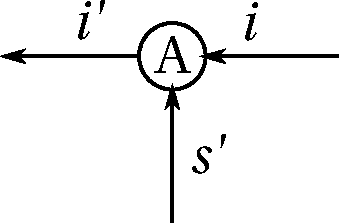
\includegraphics[width=32mm]{AMat.pdf}\par
\end{centering}

The directional arrows indicate the symmetry of the coupling coefficients.

\subsection{Bra versus ket}

An MPS constructed in this way actually looks like a bra vector, since the physical indices
are pointing inwards, which, in the conventional picture indicates a bra. This is consistent with
the quantum numbers in the auxiliary Hilbert space being 0 (vacuum) on the right-hand side
and $q$ on the left. Since the overall tensor network is a rotational invariant (scalar), the
physical quantum number is therefore the conjugate of $q$, which is correct for a bra state. The
Hermitian conjugate would correspond to a ket state with physical quantum number $q$ and
transforming as the conjugate of q in the auxiliary space.

However, we raraly need to consider mixing the physical and auxiliary Hilbert spaces, so we are free
to choose any convention we like for the physical index. Hence we are free to call it a ket.
To construct a bra vector, we will construct explicitly the Hermitian conjugate:
\beq
\braket{A}{B} \sim A^\dagger B
\eeq

Note that later on, we will see that the contraction of an MPS via $E$ and $F$-matrices, naturally leads to
$F$ being in the conjugate representation and $E$ being normal, leading to
\beq
\braket{A}{B} \sim E F^\dagger
\eeq

\subsection{Normalization}
\label{sec:AMatNormalization}

The normalization constraints for the right and left sides are
\beq
N = \sum_s \itensor{A}{s} \itensor{A^\dagger}{s}
\label{eq:staterightnorm}
\eeq
\beq
N = \sum_s \itensor{A^\dagger}{s} \itensor{A}{s}
\eeq
respectively. Typically we will want to find a transformation such
that $N = I$.
This notation arises from how we apply the matrices. If the right-hand basis
is orthonormal, then multiplying on the left by an $A$ matrix that satisfies the right orthogonality
constraint, $AA^\dagger = 1$, preserves orthonormality.  Conversely, if the left-hand basis
is orthonormal, then multiplying on the right with a left-normal matrix, $A^\dagger A = 1$, 
preserves orthonormality.
Expanding \refeq{eq:staterightnorm} in reduced matrix elements, this is
\beq
\bigbraket{j'm'}{N}{jm} = 
\sum_{s,q,j'',m''} \bigbraket{j'm'}{\itensorcomp{A}{s}{q}}{j''m''}
\bigbraket{jm}{\itensorcomp{A}{s}{q}}{j''m''}^*
\eeq

Consider first the right hand side,
\beq
\begin{array}{c}
\displaystyle
\sum_{s,j''}
\rbigbraket{j'}{\itensor{A}{s}}{j''}
\rbigbraket{j}{\itensor{A}{s}}{j''}^*
\sum_{q,m''}
\qcg{j''}{s}{j'}{m''}{q}{m'} \qcg{j''}{s}{j}{m''}{q}{m}
\\
\displaystyle
= \sum_{s,j''}
\rbigbraket{j'}{\itensor{A}{s}}{j''}
\rbigbraket{j}{\itensor{A}{s}}{j''}^*
\delta_{jj'} \delta_{mm'}
\end{array}
\eeq
which shows that $N$ is a scalar (as it should be).
Thus,
\beq
\rbigbraket{j}{N}{j} = 
\sum_{s,j''}
\rbigbraket{j}{\itensor{A}{s}}{j''}
\rbigbraket{j}{\itensor{A}{s}}{j''}^*
\eeq
because the CG coefficient that determines the reduced matrix
element of $N$ is $\qcg{j}{0}{j}{m}{0}{m} = 1$.

Alternatively, we could calculate the product
\beq
\sum_s \itensor{A^\dagger}{s} \itensor{A}{s}
\eeq
Expanding the matrix elements, this is
\beq
\bigbraket{j'm'}{N}{jm} = 
\sum_{s,q,j'',m''} \bigbraket{j''m''}{\itensorcomp{A}{s}{q}}{j'm'}^*
\bigbraket{j''m''}{\itensorcomp{A}{s}{q}}{jm}
\eeq
The CG coefficient is
\beq
\sum_{q,m''} \qcg{j'}{s}{j''}{m'}{q}{m''} \qcg{j}{s}{j''}{m}{q}{m''}
= \frac{2j''+1}{2j+1} \delta_{j'j} \delta_{m'm}
\eeq
giving the final result of
\beq
\rbigbraket{j}{N}{j} = \sum_{s,j''}
\frac{2j''+1}{2j+1}
\rbigbraket{j''}{\itensor{A}{s}}{j}^*
\rbigbraket{j''}{\itensor{A}{s}}{j}
\label{eq:LeftAMatrixNorm}
\eeq

For the center-matrix formalism, we need the transformation
\beq
\itensor{A}{s}_{ij} \rightarrow \sum_k \; C_{ik} \; \itensor{A'}{s}_{kj}
\eeq
where $k$ is a $d \times m$ dimensional index that encapsulates both a $s'$ and a $j'$ 
index\footnote{or more precisely, $k$ runs over the Clebsch-Gordan expansion
of $s' \otimes j'$.}
: $k \simeq (s',j')$.
Requiring $\itensor{A'}{s}_{kj}$ to satisfy the right orthogonality constraint,
$A' A'^{\dagger} = 1$, this requires
\beq
\itensor{A'}{s}_{kj} = \delta_{j'j}\delta_{s's} \quad \left[\mbox{with } k \simeq (s',j')\right]
\eeq
with
\beq
C_{ik} = \itensor{A}{s'}_{ij'}
\eeq

In the other direction, we need
\beq
\itensor{A}{s}_{ij} \rightarrow \sum_k \; \itensor{A'}{s}_{ik} \; C_{kj}
\eeq
where $k \simeq (s',i')$.
Requiring $\itensor{A'}{s}_{ik}$ to satisfy the left orthogonality constraint,
$A'^{\dagger} A' = 1$, this requires
\beq
\itensor{A'}{s}_{ik} = \delta_{s's} \delta_{i'i} \sqrt{\frac{2k+1}{2i+1}} 
\quad \left[\mbox{with } k \simeq (s',i')\right]
\eeq
and
\beq
C_{kj} = \itensor{A}{s}_{j'j} \sqrt{\frac{2i+1}{2k+1}}
\eeq

\subsection{MPS Contraction}
\label{sec:MPSProducts}

The contraction of MPS, given by
\beq
\itensor{F}{k} = \itensor{A}{s'} \itensor{B^\dagger}{s} \: \rbigbraket{s'}{\itensor{M}{k}}{s}
\label{eq:FMatSimple}
\eeq
is an irreducible tensor that transforms as rank $[k]$. To prove this, we expand
\beq
\begin{array}{rccl}
\rbigbraket{j'}{\itensor{F}{k}}{j} & =  \displaystyle \sum_{s's i;m n \sigma' \sigma \mu} &
& \bigbraket{j'm'}{\itensorcomp{A}{s'}{\sigma'}}{in} \\
& & \times & \bigbraket{jm}{\itensorcomp{B}{s}{\sigma}}{in}^* \\
& & \times & \bigbraket{s'\sigma'}{\itensorcomp{M}{k}{\mu}}{s\sigma} \\
& & \times & \qcg{i}{s'}{j'}{n}{\sigma'}{m'} \qcg{i}{s}{j}{n}{\sigma}{m} \\
& & \times & \qcg{s}{k}{s'}{\sigma}{\mu}{\sigma'} \qcg{j}{k}{j'}{m}{\mu}{m'}
\end{array}
\eeq
where the value of $m'$ is arbitary.  Upon the identification $i \rightarrow j_1$,
$s \rightarrow j_2$, $j \rightarrow j_{12}$, $k \rightarrow j_3$, $j' \rightarrow j'$,
$s' \rightarrow j_{23}$, we get, from \refeq{eq:SixJCG}, the relation
\beq
\begin{array}{rcl}
\rbigbraket{j'}{\itensor{F}{k}}{j} &=& \sum_{s's i} \rbigbraket{j'}{\itensor{A}{s'}}{i}
\rbigbraket{j}{\itensor{B}{s}}{i}^*
\rbigbraket{s'}{\itensor{M}{k}}{s} \\
& & \times (-1)^{i+s+k+j'} \sqrt{(2j+1)(2s'+1)} \qsixj{i}{s}{j}{k}{j'}{s'}
\end{array}
\eeq
Alternatively, we could substitute in \refeq{eq:FMatSimple} 
$\rbigbraket{s'}{\itensor{M^\dagger}{k}}{s}^*$, and we get exactly the same operator.

Another operation that we will need is when we commute the $A,B$ operators, giving
the $E$ matrix,
\beq
\itensor{E}{k} = \itensor{A^\dagger}{s'} \itensor{B}{s} \: \rbigbraket{s'}{\itensor{M^\dagger}{k}}{s}
\eeq
This is also an irreducible tensor of rank $[k]$. Expanding, we get
\beq
\begin{array}{rccl}
\rbigbraket{j'}{\itensor{E}{k}}{j} & =  \displaystyle \sum_{s's i;m n \sigma' \sigma \mu} &
& \bigbraket{in}{\itensorcomp{A}{s'}{\sigma'}}{j'm'}^* \\
& & \times & \bigbraket{in}{\itensorcomp{B}{s}{\sigma}}{jm} \\
& & \times & \bigbraket{s\sigma}{\itensorcomp{M}{k}{\mu}}{s'\sigma'}^* \\
& & \times & \qcg{j'}{s'}{i}{m'}{\sigma'}{n} \qcg{j}{s}{i}{m}{\sigma}{n} \\
& & \times & \qcg{s'}{k}{s}{\sigma'}{\mu}{\sigma} \qcg{j}{k}{j'}{m}{\mu}{m'}
\end{array}
\eeq
where again $m'$ is arbitary. Using the symmetries of the CG coefficients, we rewrite
\beq
\begin{array}{l}
\qcg{j'}{s'}{i}{m'}{\sigma'}{n} \qcg{j}{s}{i}{m}{\sigma}{n}
\qcg{s'}{k}{s}{\sigma'}{\mu}{\sigma}
= \\
(-1)^{s'+\sigma'}
\sqrt{\frac{2i+1}{2j'+1}}
\qcg{i}{s'}{j'}{-n}{\sigma'}{-m'}
%
(-1)^{s+\sigma}
\sqrt{\frac{2i+1}{2j+1}}
\qcg{i}{s}{j}{-n}{\sigma}{-m}
%
(-1)^{k+\mu}
\sqrt{\frac{2s+1}{2s'+1}}
\qcg{s}{k}{s'}{-\sigma}{\mu}{-\sigma'}
\end{array}
\eeq
We are free to change the sign of the dummy indices $\sigma', \sigma$, which then gives
the same set of CG coefficients that we had previously, except for a factor which we can
write as
\beq
(-1)^{\sigma'+\mu-\sigma}(-1)^{s'+k-s} 
\frac{2i+1}{2j'+1} \sqrt{\frac{2j'+1}{2j+1}} \sqrt{\frac{2s+1}{2s'+1}} \; .
\eeq
Since, with our negated dummy indices, $\sigma = \sigma'+\mu$, we get
\beq
\begin{array}{rcl}
\rbigbraket{j'}{\itensor{E}{k}}{j} &=& \sum_{s's i} \rbigbraket{i}{\itensor{A}{s'}}{j'}^*
\rbigbraket{i}{\itensor{B}{s}}{j}
\rbigbraket{s'}{\itensor{M^\dagger}{k}}{s} \\
& & \times (-1)^{i+s'+k+j} \sqrt{(2j'+1)(2s+1)} \qsixj{i}{s}{j}{k}{j'}{s'} \\
& & \times (-1)^{j'+k-j} \frac{2i+1}{2j'+1}
\end{array}
\eeq
Which we can see as similar to \refeq{eq:FMatSimple}.

\section{Matrix Product Operators}

The most natural definition for a matrix product operator has two downstairs indices
and three upstairs,
\beq
M^{[k]}_{s'i'} {}^{si}
\eeq
which transforms as the product of two operators of rank $[k]$, with matrix elements
\beq
\bigbraket{s'q' ; j'm'}{\itensorcomp{M}{k}{r}}{sq ; jm}
= \rbigbraket{s';j'}{\itensor{M}{k}}{s;j} \; \qcg{s}{k}{s'}{q}{r}{q'} \;
\qcg{j}{k}{j'}{m}{r}{m'}
\label{eq:MPODef}
\eeq

This has the form

\begin{centering}
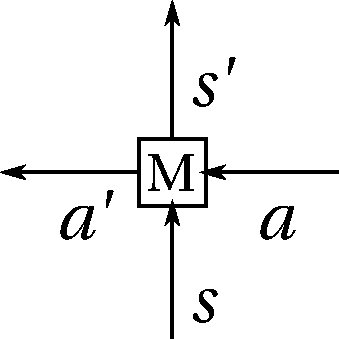
\includegraphics[width=32mm]{MPO.pdf}\par
\end{centering}


\subsection{Normalization}

The normalization conditions are
\beq
\begin{array}{rcl}
N & = & \Tr_{k} \itensor{M}{k} \itensordag{M}{k} \\
N & = & \Tr_{k} \itensordag{M}{k} \itensor{M}{k}
\end{array}
\eeq
where we take here the product with respect to both the local and
auxilary indices, and trace over the local index. This gives
\beq
\rbigbraket{j}{N}{j} = \sum_{s',s,j'',k}
(2s'+1)
\rbigbraket{j;s'}{\itensor{M}{k}}{j'';s}
\rbigbraket{j;s'}{\itensor{M}{k}}{j'';s}^*
\eeq
or,
\beq
\rbigbraket{j}{N}{j} = \sum_{s',s,j'',k}
\frac{(2j''+1)(2s'+1)}{2j+1}
\rbigbraket{j'';s'}{\itensor{M}{k}}{j;s}^*
\rbigbraket{j'';s'}{\itensor{M}{k}}{j;s}
\eeq

\subsection{Operator-State Product}

Note that the product of an operator and a state requires
a contraction of the index $s$, which has the symmetry of
over two \textit{downstairs} indices, and then shifting the result index $s'$ 
from upstairs to downstairs. For $SU(2)$, the required phase factor is
$(-1)^{s+k-s'}$, giving the rule
\beq
\itensor{B}{s'} = \itensor{(MA)}{s'} 
= \sum_s (-1)^{s+k-s'} \itensor{M}{k}^{s's} \otimes \itensor{A}{s}
\label{eq:OperatorStateProduct}
\eeq
We can prove this in a variety of ways, here I take the long but solid approach
of reverting to the definition of the reduced matrix elements.
We apply an operator to a state by contracting over the $s$ index, and
taking the tensor product of the matrices,
\beq
\begin{array}{l}
\bigbraket{j'_1 j'_2 ; m'_1 m'_2}{\itensorcomp{B}{s'}{q'}}{j_1 j_2 ; m_1 m_2}
\\ \quad \quad \displaystyle
= \sum_{s,q,k,r} \bigbraket{s'q' ; j'_1 m'_1}{\itensorcomp{M}{k}{r}}{sq ; j_1 m_1}
\bigbraket{j'_2 m'_2}{\itensorcomp{A}{s}{q}}{j_2 m_2}
\end{array}
\eeq
Now we couple $j'_1, j'_2 \rightarrow j'$ and $j_1, j_2 \rightarrow j$,
to get the reduced matrix elements of $B$;
\beq
\begin{array}{l}
\rbigbraket{(j'_1 j'_2)j'}{\itensor{B}{s'}}{(j_1 j_2)j}
= \sum_{
j'_1 m'_1 j'_2 m'_2 \;
j_1 m_1 j_2 m_2 \;
m q}
\\ \quad \quad
\qcg{j'_1}{j'_2}{j}{m'_1}{m'_2}{m'} \qcg{j_1}{j_2}{j}{m_1}{m_2}{m}
\qcg{j}{s'}{j'}{m}{q'}{m'} 
% \\ && \quad \times
\bigbraket{j'_1 j'_2 ; m'_1 m'_2}{\itensorcomp{B}{s'}{q'}}{j_1 j_2 ; m_1 m_2}
\end{array}
\eeq
where $m'$ is arbitrary. Now expanding $B$ in terms of the reduced matrix
elements of $M$ and $A$,
\beq
\begin{array}{l}
\rbigbraket{(j'_1 j'_2)j'}{\itensor{B}{s'}}{(j_1 j_2)j}
= \sum \:
\qcg{j'_1}{j'_2}{j'}{m'_1}{m'_2}{m'} \qcg{j_1}{j_2}{j}{m_1}{m_2}{m}
\qcg{j}{s'}{j'}{m}{q'}{m'} 
\\ \quad \quad \times \:
\qcg{s}{k}{s'}{q}{r}{q'} \qcg{j_1}{k}{j'_1}{m_1}{r}{m'_1}
\qcg{j_2}{s}{j'_2}{m_2}{q}{m'_2}
\\ \quad \quad \times \:
\rbigbraket{s' ; j_1'}{\itensor{M}{k}}{s ; j_1}
\rbigbraket{j'_2}{\itensor{A}{s}}{j_2}
\end{array}
\eeq

On making the transformation 
$\qcg{s}{k}{s'}{q}{r}{q'} = (-1)^{s+k-s'} \qcg{k}{s}{s'}{r}{q}{q'}$, and 
substituting
\beq
\begin{array}{rcl}
k & \rightarrow & j_{3} \\
s & \rightarrow & j_{4} \\
s' & \rightarrow & j_{34} \\
j'_1 & \rightarrow & j_{13} \\
j'_2 & \rightarrow & j_{24} \\
j' & \rightarrow & j \\
\end{array}
\eeq
we obtain immediately the $[\cdots]$ coefficient from \refeq{eq:NineJSqDef}
(remembering that there is no summation over $m$ or $m'$ in either equation),
modified by the phase $(-1)^{s+k-s'}$. Thus,
\beq
\itensor{(MA)}{s'} = \sum_s (-1)^{s+k-s'} 
\itensor{M}{k}^{s's} \otimes \itensor{A}{s}
\eeq

\begin{centering}
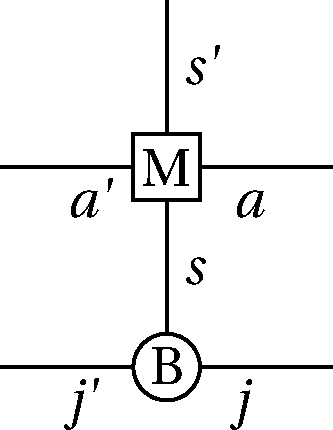
\includegraphics[width=32mm]{ApplyMB.pdf}\par
\end{centering}

This corresponds to
\beq
B'^{s'}_{(j'a'),(ja)} = M^{s's}_{a'a} B^s_{j'j}
\eeq

The matrix elements are
\beq
\bigbraket{i'\iota';a'\alpha'}{\itensorcomp{B'}{s'}{\sigma'}}{i\iota;a\alpha}
= \sum_{s\sigma k r}
\bigbraket{s'a' ; \sigma'\alpha'}{\itensorcomp{\bar{M}}{k}{r}}{sa ; \sigma\alpha}
\bigbraket{i'\iota'}{\itensorcomp{B}{s}{\sigma}}{i\iota}
\eeq
In terms of the reduced matrix elements, the right hand side is
\beq
(-1)^{s'+k-s}\sqrt{\frac{2s'+1}{2s+1}}
\qcg{s'}{k}{s}{\sigma'}{r}{\sigma}
\qcg{a}{k}{a'}{\alpha}{r}{\alpha'}
\rbigbraket{s';a'}{\itensor{M}{k}}{s;a} \:
\qcg{i}{s}{i'}{\iota}{\sigma}{\iota'} \rbigbraket{i'}{\itensor{B}{s}}{i}
\eeq
and we want to couple $(i'a') \rightarrow j'$ and $(ia) \rightarrow j$, which gives additional CG coefficients,
\beq
\qcg{i'}{a'}{j'}{\iota'}{\alpha'}{m'}
\qcg{i}{a}{j}{\iota}{\alpha}{m}
\eeq
and we want to write the final result as
\beq
\rbigbraket{j'}{\itensor{B'}{s'}}{j} 
=
\sum_{m'\sigma' m} \frac{1}{2j'+1}
\bigbraket{j'm'}{\itensorcomp{B'}{s'}{\sigma'}}{jm}
\qcg{j}{s'}{j'}{m}{\sigma'}{m'}
\eeq




\subsection{Operator-Operator Product}

The action of a matrix-product operator on another matrix product
operator is
\beq
\itensor{X}{x} = \itensor{M}{m} \itensor{N}{n}
\eeq
which corresponds to the ordinary (contraction) product in the local
basis and the tensor product in the auxiliary basis.

\subsection{Operator Adjoint}

Previous versions of these notes included a section on the MPO adjoint; this is now superseded by
the section on Hermitian conjugation above. But we note (1) the flip conjugation operation used
to be defined without the phase factor - this is unphysical in some sense but is how the toolkit 
defines it (as of 2015/09/08), and (2) there was an error in the phase factor in the old notes,
with a footnote that the toolkit (and my thesis) implemented it differently. In fact the error
was in these notes, which is now fixed.

\subsection{Operator product}

For the evaluation of matrix elements, we need the operation
\beq
F^{a'}_{i'j'} = \sum_{s',s,i,j,a}
{M}^{s's}_{a'a} {A}^{*s'}_{i'i} {B}^{s}_{j'j} 
{E}^{a}_{ij}
\eeq
On expanding out the reduced matrix elements, we see immediately that the
coupling coefficient is
\beq
\itensor{F}{a'}_{i'j'} =
\sum_{a,i,j,k,s,s'}
\qninejsq{j}{s}{j'}{a}{k}{a'}{i}{s'}{i'}
%{j}{a}{i}{s}{k}{s'}{j'}{a'}{i'}
\itensor{M}{k}^{s's}_{a'a} \itensor{A}{s'}^*_{i'i} \itensor{B}{s}_{j'j} 
\itensor{E}{a}_{ij}
\eeq

Conversely, from the left hand side,
\beq
F^{a}_{ij} = \sum_{s',s,i',j',a'}
E^{a'}_{i'j'} M^{s's}_{a'a} A^{*s'}_{i'i} B^{s}_{j'j}
\eeq
is
\beq
\itensor{F}{a}_{ij} = \sum_{a',i',j',k,s',s}
\frac{2i'+1}{2i+1}
\qninejsq{j}{s}{j'}{a}{k}{a'}{i}{s'}{i'}
\itensor{E}{a'}_{i'j'}
\itensor{M}{k}^{s's}_{a'a} \itensor{A}{s'}^*_{i'i} \itensor{B}{s}_{j'j}
\eeq

On interchanging $A \leftrightarrow E$, $B \leftrightarrow F$, 
this becomes the equation
for a direct operator-matrix-product multiply. But using the center-matrix
formalism, we want instead the operation
\beq
\psi'_{i'i} = \sum_{k'kj'j} E^{k'}_{i'j'}  F^{k}_{ij} H_{k'k} \psi_{j'j}
\eeq
where $\psi$, $\psi'$, and $H$ transform as scalars, \ie
the quantum numbers impose $i'=i$, $j'=j$, $k'=k$. $H$ is the center
matrix of the operator, and $\psi$ is the center matrix of the wavefunction.
This is essentially the scalar product $E \cdot F$, and the coupling coefficients
drop out. 

For an overlap, the usual scaling applies,
\beq
\braket{A}{B} = \sum_{i'i} (2i'+1) A^*_{i'i} B_{i'i}
\eeq
which reduces the full overlap equation $\bigbraket{A}{M}{B}$ to
\beq
\sum_{i'ik'k} (2i'+1)
A^*_{i'i} E^{k'}_{i'j'} F^{k}_{ij} H_{k'k} B_{j'j}
\eeq

\subsection{Alternate notation}

It may be better to use the notation of \refsec{sec:MPSProducts}. We want to construct
\beq
\itensor{F'}{a'} = \itensor{A}{s'} \itensor{F}{a} \itensor{B^\dagger}{s} \: 
\rbigbraket{s';a'}{\itensor{M}{k}}{s;a}
\label{eq:FMat}
\eeq
The reduced matrix elements of the right hand side are
\beq
\rbigbraket{j'}{\itensor{A}{s'}}{i'}
\rbigbraket{i'}{\itensor{F}{a}}{i}
\rbigbraket{i}{\itensor{B^\dagger}{s}}{j}
\rbigbraket{s';a'}{\itensor{M}{k}}{s;a}
\eeq
which leads to the reduced matrix elements $\rbigbraket{j'}{\itensor{F'}{a'}}{j}$, 
via the coefficients
\beq
\sum_{\sigma'\sigma n' n \alpha' \alpha m M}
\qcg{i'}{s'}{j'}{n'}{\sigma'}{m'}
\qcg{i}{a}{i'}{n'}{\alpha'}{n'}
\qcg{i}{s}{j}{n}{\sigma}{m}
\qcg{s}{k}{s'}{\sigma}{M}{\sigma'}
\qcg{a}{k}{a'}{\alpha}{M}{\alpha'}
\qcg{j}{a'}{j'}{m}{\alpha'}{m'}
\eeq
where the value of $m'$ is arbitary.
Upon identifying $i \rightarrow j_1$, $s \rightarrow j_2$, $j \rightarrow j_{12}$,
$a \rightarrow j_3$, $k \rightarrow j_4$, $a' \rightarrow j_{34}$,
$i' \rightarrow j_{13}$, $s' \rightarrow j_{24}$, $j' \rightarrow j$,
we get immediately
\beq
\begin{array}{rcl}
\rbigbraket{j'}{\itensor{F'}{a'}}{j}
&=& 
\rbigbraket{j'}{\itensor{A}{s'}}{i'}
\rbigbraket{i'}{\itensor{F}{a}}{i}
\rbigbraket{j}{\itensor{B}{s}}{i}^* \:
\rbigbraket{s';a'}{\itensor{M}{k}}{s;a}
\\
& & \quad \times
\qninejsq{i}{s}{j}{a}{k}{a'}{i'}{s'}{j'}
\end{array}
\eeq
Compare with the triple product formula, in \refeq{eq:TripleProdF}.

The corresponding $E$ operator is
\beq
\itensor{E}{a} = \itensor{A^\dagger}{s'} \itensor{E'}{a'} \itensor{B}{s} \: 
\rbigbraket{s;a}{\itensor{M^\dagger}{k}}{s';a'}
\label{eq:EMat}
\eeq
The matrix elements are
\beq
\begin{array}{rcl}
\rbigbraket{j'}{\itensor{E}{e}}{j} 
&=& \displaystyle
\frac{1}{2j'+1} \sum_{mm'nn'\sigma\sigma'aa'M}
\rbigbraket{i'}{\itensor{A}{s'}}{j'}^* \:
\rbigbraket{i'}{\itensor{E'}{a'}}{i}
\rbigbraket{i}{\itensor{B}{s}}{j}
\rbigbraket{s';a'}{\itensor{M}{k}}{s;a}^*
\\ 
&& \quad \times \: 
\qcg{j'}{s'}{i'}{m'}{\sigma'}{n'}
\qcg{i}{a'}{i'}{n'}{\alpha'}{n'}
\qcg{j}{s}{i}{m}{\sigma}{n}
\qcg{s}{k}{s'}{\sigma}{M}{\sigma'}
\qcg{a}{k}{a'}{\alpha}{M}{\alpha'}
\qcg{j}{a'}{j'}{m}{\alpha'}{m'}
\end{array}
\eeq
from which we identify $j \rightarrow j_1$, $s \rightarrow j_2$, $i \rightarrow j_{12}$,
$a \rightarrow j_3$, $k \rightarrow j_4$, $a' \rightarrow j_{34}$,
$j' \rightarrow j_{13}$, $s' \rightarrow j_{24}$, $i' \rightarrow j$,
to give
\beq
\begin{array}{rcl}
\rbigbraket{j'}{\itensor{E}{e}}{j} 
&=& \displaystyle
\rbigbraket{i'}{\itensor{A}{s'}}{j'}^* \:
\rbigbraket{i'}{\itensor{E'}{a'}}{i}
\rbigbraket{i}{\itensor{B}{s}}{j}
\rbigbraket{s';a'}{\itensor{M}{k}}{s;a}^*
\\
&& \displaystyle \quad \times \: 
\frac{2i'+1}{2j'+1}
\qninejsq{j}{s}{i}{a}{k}{a'}{j'}{s'}{i'}
\end{array}
\eeq
Compare with the triple product formula, in \refeq{eq:TripleProdE}.

A note on this notation: we have chosen here to have the Hermitian conjugate appear in the
$E$ matrix definition, and not in the $F$ matrix. This is consistent in the sense that
if we accumulate tensors coming from both the left and the right, the final expectation
value is $\Tr \itensor{E^\dagger}{a} \itensor{F}{a}$. \textbf{should check this!}

\section{Matrix-vector multiply}

If we are not using the center-matrix formalism, then we need to apply the $E$ and $F$ matrices
directly to an MPS. This operation is
\beq
A'^{s'}_{ij} = M^{s's}_{a'a} E^{*a'}_{i'i} A^s_{i'j'} F^{a}_{j'j}
\eeq
Since we are treating the local basis elements in $A$ as downstairs indices, we expect
similar conjugate phase issues as for the operator-state product.


% Result[s'](i',i) = M(s',s)[a',a] herm(E[a'](i',j')) herm(B[s](j',j)) F[a](i,j)

A contraction that we want to perform is
\beq
A^{s'}_{i'i} =  M^{s',s}_{a'a}E^{a'\dagger}_{i'j'} F^a_{ij} B^{s\dagger}_{j'j}
\eeq
To construct the coupling coefficient, we write the matrix elements, which gives the
quantum number triples
\beq
(j,s,j') (j,a,i) (j',a',i') (a,k,a') (s,k,s') \rightarrow (i,s',i')
\eeq
We can identify this with the $9j$ coefficient,
\beq
\rbigbraket{i'}{\itensor{A}{s'}}{i} =
\qninejsq{j}{s}{j'}{a}{k}{a'}{i}{s'}{i'}
\rbigbraket{s';a'}{\itensor{M}{k}}{s;a}
\bigbraket{i'}{\itensor{E}{a'}}{j'}^*
\bigbraket{i}{\itensor{F}{a}}{j}
\bigbraket{j'}{\itensor{B}{s}}{j}^*
\eeq



\subsection{E-matrix}

We can express the E-matrix contraction as

\begin{centering}
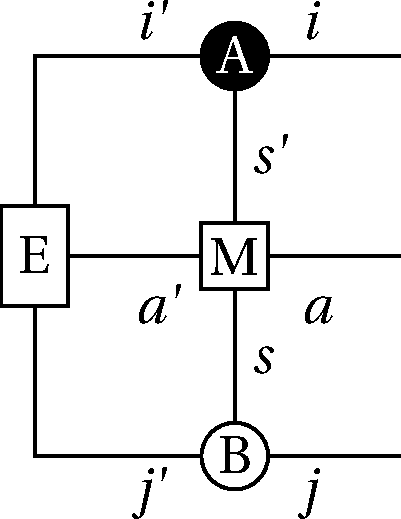
\includegraphics[width=32mm]{EMat.pdf}\par
\end{centering}

This has two incoming indices, and one out index, and therefore transforms as an ordinary tensor,
\beq
E'^{a}_{ij} = M^{s's}_{a'a} \bar{B}^s_{i'i} E^{a'}_{i'j'} A^{s'}_{j'j} 
\eeq

\subsection{F-matrix}

The F-matrix is the contraction from the other side:

\begin{centering}
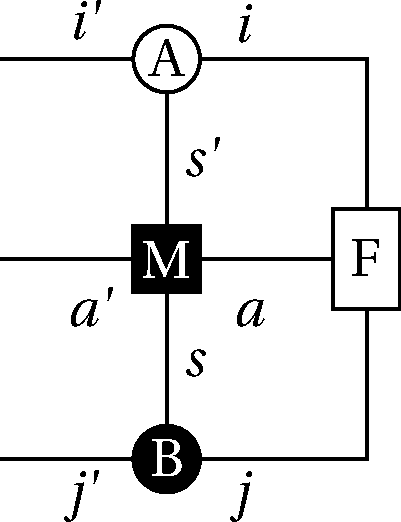
\includegraphics[width=32mm]{FMat.pdf}\par
\end{centering}

This has two outgoing indices and one in index, and therefore transforms as a conjugate tensor. Hence
the tensor that we will actually obtain is $\bar{F}$, which is obtained as
\beq
\bar{F'}^{a'}_{i'j'} = M^{s's}_{a'a} \bar{B}^s_{i'i} A^{s'}_{j'j} \bar{F}^a_{ij}
\eeq
Or, conjugating all tensors,
\beq
F'^{a'}_{i'j'} = \bar{M}^{s's}_{a'a} B^s_{i'i} \bar{A}^{s'}_{j'j} F^a_{ij}
\eeq


\section{Direct SVD}

We want to calculate the SVD directly of A-matrices, for the 1-site algorithm,
and also for a pair of A-matrices for the 2-site algorithm,

\subsection{Single matrix, truncating basis 2}

Here we consider the decomposition of an A-matrix into 
\beq
A^s = X = U^s D V
\eeq
where we treat $X$ as a $dm\times m$ matrix.
For the subspace expansion technique, $A^s$ is expanded on the right-hand side
to be $m'$ states, so that $X$ is $dm \times m'$, then we have
$U^s$ as $d\times m\times m'$, and $D. V$ are $m' \times m'$.

This is essentially the same operation that we did in the center-matrix formulation.
Phase factors appearing in X are irrelevant since they will cancel out again when
we convert back into $U^s$. Hence section \refsec{sec:AMatNormalization} applies,
and we can write $A^s = A^{'s} X$, where $A^{'s}$ is a $d \times m \times dm$ 
MPS that satisfies the left orthogonality constraint, $A^{'\dagger}A'=I$. This gives
\beq
X^{ji} = A^{s}_{i'i} \sqrt{\frac{2i'+1}{2i+1}}
\eeq
where $j = (i'\bar{s})$. The reverse of this is
\beq
A^{s}_{i'i} = X_{ji} \sqrt{\frac{2i+1}{2i'+1}}
\eeq

% To construct the matrix $X$, we must write $A^s$ as a scalar operator, where the $s$ index
% acts on the left. This will necessarily be the adjoint quantum number. The matrix elements
% are
% \beq
% \bigbraket{(i'\bar{s})(\iota'\sigma')}{\itensorcomp{A}{0}{0}}{i\iota} 
% = \qcg{i}{0}{i}{\iota}{0}{\iota} \qcg{i'}{\bar{s}}{i}{\iota'}{-\sigma}{i} 
% \rbigbraket{(i'\bar{s})}{\itensor{A}{0}}{i}
% \eeq
% We want the left hand side to be equal to the matrix elements of $A^s$,
% \beq
% \bigbraket{(i'\bar{s})(\iota'\sigma')}{\itensorcomp{A}{0}{0}}{i\iota} 
% = 
% \bigbraket{i'\iota'}{\itensorcomp{A}{s}{-\sigma}}{i\iota} 
% \eeq
% Using the symmetry relations,
% \beq
%  \qcg{i'}{\bar{s}}{i}{\iota'}{-\sigma}{i} =
% (-1)^{s+\sigma}\sqrt{\frac{2i+1}{2i'+1}} \qcg{i}{\bar{s}}{i'}{-\iota}{-\sigma}{-\iota'}
% = (-1)^{i+s-i'} (-1)^{s+\sigma}\sqrt{\frac{2i+1}{2i'+1}} \qcg{i}{\bar{s}}{i'}{\iota}{\sigma}{\iota'}
% \eeq



\subsection{Single matrix, truncating basis 1}

Here we consider the decomposition of an A-matrix into 
\beq
A^s = X = U D V^s
\eeq
where we treat $X$ as a $m\times dm$ matrix.
For the subspace expansion technique, $A^s$ is expanded on the left-hand side
to be $m'$ states, so that $X$ is $m' \times dm$, then we have
$V^s$ as $d\times m'\times m$, and $U, D$ are $m' \times m'$.

In writing $A^s$ as a scalar operator, we need to get the coupling coefficients correct
because the same index on the right of $A^s$ can appear in more than one $s$ sector.
The matrix elements of $A^s$ are
\beq
\bigbraket{i'\iota'}{\itensorcomp{A}{s}{\sigma}}{i\iota} 
= \qcg{i}{s}{i'}{\iota}{\sigma}{\iota'}
\rbigbraket{i'}{\itensor{A}{s}}{i}
\eeq
Converting this into a scalar by coupling spins $i,s$ to spin $i'$, gives 
\beq
\bigbraket{i'}{\itensorcomp{A}{0}{0}}{i'(is)} = 
\qcg{i'}{0}{i'}{\iota'}{0}{\iota'} \qcg{i}{s}{i'}{\iota}{\sigma}{\iota'}
\rbigbraket{i'}{\itensor{A}{0}}{i'(is)}
\eeq
The coupling coefficient for mapping $(i,s)$ into $i'$ coincides with that of the
original reduced matrix element, which is convenient. The extra term is $\qcg{i'}{0}{i'}{\iota'}{0}{\iota'}$
which is identically 1, from \refeq{eq:CG_SpecialCase}. Hence we have
\beq
\rbigbraket{i'}{\itensor{A}{0}}{i'(is)} = \rbigbraket{i'}{\itensor{A}{s}}{i}
\eeq

\subsection{Direct SVD of two MPS}

For two-site algorithms that act on the A-matrices directly, we need to combine the two sites 
into one (which is a simple multiplication of the A-matrices using \refeq{eq:TensorProduct}),
and then decompose this back into two A-matrices with a singular value decomposition.
To do this decomposition, we multiply both sites of \refeq{eq:TensorProduct} by
\beq
(-1)^{j+j'+k} \sqrt{(2r+1)(2k+1)} \qsixj{j'}{k_1}{r}{k_2}{j}{k}
\eeq
and sum over $k$. Using the orthogonality constraint \refeq{eq:6jortho} this gives
\beq
\begin{array}{l}
\rbigbraket{j'}{\itensor{S}{k_1}}{r}
\rbigbraket{r}{\itensor{T}{k_2}}{j} \\ \quad
= (-1)^{j+j'+k} \sum_{k} \sqrt{(2r+1)(2k+1)} \qsixj{j'}{k_1}{r}{k_2}{j}{k}
\\ \quad \quad \times
\rbigbraket{j'}{\left[ \itensor{S}{k_1} \times \itensor{T}{k_2} \right]^{[k]}}{j}
\end{array}
\eeq
which is pleasingly symmetric with \refeq{eq:TensorProduct}.


\section{Delta Shifts}

When inserting sites into a MPS we want to manipulate the quantum number of the target state.
This operation corresponds to inserting an operator that transforms as $k$ (ie. the quantum
number of the inserted sites) which we need to apply to all tensors to the left, and then
project onto the desired new target state for the full system.

In the case where the $SU(2)$ quantum number strictly \textit{increases}, this has a simplified
form, because then the basis size is unchanged; each state $j$ simply 
shifts $j \rightarrow j + \Delta$. Clearly we cannot do this if $j+\Delta$ is negative, but
the common case will be, eg, fixed magnetization per site, in which case $\Delta \geq 0$.
We refer to this as a \textit{$\Delta$-shift}, it corresponds to the application of
a \textit{unit tensor operator} \cite{BiedenharnVol2}.

The effect is the same as tensor product with an $m=1$ identity operator, with
only one non-zero matrix element $\rbigbraket{\Delta}{\itensor{M}{0}}{\Delta}$.
In the tensor product we want to take only the basis states in the heightest weight, 
$D(j) \otimes D(\Delta) \rightarrow D(j + \Delta)$.
This is equation \refeq{eq:OperatorStateProduct} with \refeq{eq:TensorProductCoupling}
restricted to a single $j',j$.
The phase factor from \refeq{eq:OperatorStateProduct} vanishes leaving a matrix element
\beq
\begin{array}{l}
\rbigbraket{j'+\Delta}{\itensor{M}{0} \otimes \itensor{A}{k}}{j+\Delta} \\
= \rbigbraket{\Delta}{\itensor{M}{0}}{\Delta} \rbigbraket{j'}{\itensor{A}{k}}{j}
\qninejsq{\Delta}{j}{j+\Delta}{0}{k}{k}{\Delta}{j'}{j'+\Delta}
\end{array}
\eeq
Making use of the zero to reduce this to a $6j$ coefficient, the coupling coefficient
is (need to verify this!)
\beq
\begin{array}{rcl}
\qninejsq{\Delta}{j}{j+\Delta}{0}{k}{k}{\Delta}{j'}{j'+\Delta}
&=& (-1)^{(j+\Delta)+k+\Delta+j'} \sqrt{(2j+2\Delta+1)(2j'+1)}
\\ & & \quad \times
\qsixj{j}{j'}{k}{j'+\Delta}{j+\Delta}{\Delta}
\end{array}
\eeq

Unfortunately, this approach does not work: the effect of applying an $m=1$ identity operator
and projecting onto some target $j+\Delta$ state is not equivalent to applying the $\Delta$ shift
to each $A$-matrix. Consider the left-most $A$-matrix, where the left basis is one-dimensional
and represents the target state. Without restricting the right basis, the product coefficient is
\beq
\qninejsq{\Delta}{j}{j+a}{0}{k}{k}{\Delta}{j'}{j'+\Delta}
\eeq
where $a$ is the quantum number in the right basis. The restrictions on the possible values
of $a$ arise from the need to satisfy the triangle constraints for the first row and third column.
This gives $|j-\Delta| \leq a \leq j+\Delta$ and $|j'+\Delta-k| \leq a \leq j'+\Delta+k$.
Thus, in general, more than one $a$ will satisfy these constraints. We can understand this by
viewing the $\Delta$-shift as a two-step operation; firstly we apply the $m=1$ operator, which gives
up to $2\Delta+1$ target states; at this point the $A$-matrices will preserve whatever normalization
constraints they had previously. Follow this by a projection onto a single target state. As for any
form of projection, this does not preserve the normalization.

The question remains: can we get away with a $\Delta$-shift followed by a reorthogonalization of
the basis? Or do we need, as suggested above, to include all states? How can we have an (approximately)
translationally invariant state if we need to include all states, as this would magnify the basis
size for higher quantum numbers?

\section{Translation MPO}

In this section, we deduce the MPO representation for the translation operator
that shifts sites to the left or right. 

\subsection{Right translation}

Here we define a
right translation, that is an operator that acts on a wavefunction so that
the site originally labelled site 0 becomes site 1 after the shift.
In the notation of \refeq{eq:MPODef}, this has the form

\beq
\rbigbraket{s';j'}{\itensor{T_R}{k}}{s;j} = \delta_{s' j'} \delta_{s j} \epsilon_{sks'}
\frac{2k+1}{2s+1} 
\eeq
where $k$ takes on all values that satisfy the triangle condition
$\epsilon_{sks'}=1$.

To prove this, we construct the full matrix elements,
\beq
\bigbraket{s'q' ; j'm'}{\itensorcomp{T_R}{k}{r}}{sq ; jm}
= \delta_{s' j'} \delta_{s j} \epsilon_{sks'} \; \qcg{s}{k}{s'}{q}{r}{q'} \;
\qcg{j}{k}{j'}{m}{r}{m'} \frac{2k+1}{2s+1}
\eeq
To obtain the physical matrix elements we sum over $k$, $r$, and make use of the
orthogonality of columns of the Clebsch-Gordan coefficients,
\beq
\qcg{s}{k}{s'}{q}{r}{q'} \; \qcg{j}{k}{j'}{m}{r}{m'}
=  (-1)^{s-q} \sqrt\frac{2s+1}{2k+1} \qcg{s}{s'}{k}{q}{-q'}{-r}
(-1)^{j-m} \sqrt\frac{2j+1}{2k+1} \qcg{j}{j'}{k}{m}{-m'}{-r}
\eeq
Thus
\beq
\sum_{k,r}  \delta_{s' j'} \delta_{s j} \epsilon_{sks'}
(-1)^{2s-q-m}  \qcg{s}{s'}{k}{q}{-q'}{-r} \qcg{j}{j'}{k}{m}{-m'}{-r}
= (-1)^{2s-q-m} \delta_{s' j'} \delta_{s j} \delta_{q' m'} \delta_{q m}
\eeq
The phase factor out the front vanishes: $s$ and $q$ are either both
integer or both odd-half-integer, so $s-q$ is always integer, and $2(s-q)$ is always
even. And finally,
\beq
\bigbraket{s'q' ; j'm'}{\itensorcomp{T_R}{k}{r}}{sq ; jm}
= \delta_{s' j'} \delta_{s j} \epsilon_{sks'} \; \delta_{q' m'} \delta_{q m}
\eeq
as expected.

\subsection{Left translation}

Here we define a
left translation, that is an operator that acts on a wavefunction so that
the site originally labelled site 1 becomes site 0 after the shift.
In the notation of \refeq{eq:MPODef}, this has the form
\beq
\rbigbraket{s';j'}{\itensor{T_L}{k}}{s;j} = \delta_{s' j} \delta_{s j'} \epsilon_{sks'}
\frac{2k+1}{2s+1}
\eeq
The full matrix elements are
\beq
\bigbraket{s'q' ; j' -m'}{\itensorcomp{T_R}{k}{r}}{sq ; j -m}
= \delta_{s' j} \delta_{s j'} \epsilon_{sks'} \;
\frac{2k+1}{2s+1}
 \qcg{s}{k}{s'}{q}{r}{q'} \;
\qcg{s'}{k}{s}{-m}{r}{-m'}
\eeq
Using the symmetries of the Clebsch-Gordan coefficients,
\beq
\bigbraket{s'q' ; j'm'}{\itensorcomp{T_R}{k}{r}}{sq ; jm}
= \delta_{s' j} \delta_{s j'} \epsilon_{sks'} \; 
\frac{2k+1}{2s+1}
(-1)^{s-q} \sqrt\frac{2s+1}{2k+1} \qcg{s}{s'}{k}{q}{-q'}{-r} \;
(-1)^{s'+m} \sqrt\frac{2s+1}{2k+1} (-1)^{s+s'-k} \qcg{s}{s'}{k}{m'}{-m}{-r}
\eeq
\beq
= \delta_{s' j} \delta_{s j'} \epsilon_{sks'}  
(-1)^{k-q+m} \qcg{s}{s'}{k}{q}{-q'}{-r} \qcg{s}{s'}{k}{m'}{-m}{-r}
\eeq
Summing over $k$, $r$, and using the orthogonality of columns,
\beq
= \delta_{s' j} \delta_{s j'} \epsilon_{sks'} \delta_{q,m'} 
\delta_{q',m} (-1)^{k-m'+m}

\eeq

\section{Partial transpose}

(incomplete)

For the calculation of exponents of operators, we need the partial transpose operation. Writing
the matrix elements of $M$ as
\begin{equation}
\rbigbraket{a'}{\itensor{M}{k}}{a}
\end{equation}
where the $a',a$ indices have a tensor decomposition,
\begin{equation}
\begin{array}{rcl}
\rket{a'} &=& \rket{j_1} \rket{j_2} \\
\rket{a} &=& \rket{i_1} \rket{i_2}
\end{array}
\end{equation}
this gives the reduced matrix elements
\begin{equation}
\rbigbraket{(i_1 i_2) a'}{\itensor{M}{k}}{(j_1 j_2) a} \; ,
\end{equation}
which has reduced matrix elements
\begin{equation}
\qcg{i_1}{i_2}{a'}{m_1}{m_2}{\alpha'}
\qcg{j_1}{j_2}{a}{n_1}{n_2}{\alpha}
\qcg{a}{k}{a'}{\alpha}{q}{\alpha'}
\bigbraket{(i_1, n_1 ; i_2, n_2) a',\alpha'}{\itensorcomp{M}{k}{q}}{(j_1,n_1;j_2,n_2) a,\alpha}
\end{equation}

Now we want to do a partial transpose, to write
\begin{equation}
\rbigbraket{(i_1 j_1) a_1}{\itensor{M^{PT}}{k}}{(i_2 j_2) a_2}
\label{eq:TransposedRME}
\end{equation}
which has reduced matrix elements
\begin{equation}
\qcg{i_1}{j_1}{a_1}{n_1}{m_1}{\alpha_1}
\qcg{i_2}{j_2}{a_2}{n_2}{m_2}{\alpha_2}
\qcg{a_2}{k}{a_1}{\alpha_2}{q}{\alpha_1}
\rbigbraket{(i_1,n_1; j_1,m_1) a_1,\alpha_1}{\itensorcomp{M^{PT}}{k}{q}}{(i_2,n_2; j_2,m_2) a_2,\alpha_2}
\end{equation}

Starting from \refeq{eq:TransposedRME}, we write the reduced matrix element as
\begin{equation}
\begin{array}{l}
\displaystyle
\rbigbraket{(i_1 j_1) a_1}{\itensor{M^{PT}}{k}}{(i_2 j_2) a_2} \\ \quad \displaystyle
= \frac{1}{2a_1+1} \sum_{\alpha_1 q \alpha_2} \qcg{a_2}{k}{a_1}{\alpha_2}{q}{\alpha_1}
\rbigbraket{a_1,\alpha_1}{\itensorcomp{M^{PT}}{k}{q}}{a_2,\alpha_2} \\ \quad \displaystyle
= \frac{1}{2a_1+1} \sum_{\alpha_1 q \alpha_2} \sum_{m_1 m_2 n_1 n_2}
\qcg{i_1}{j_1}{a_1}{n_1}{m_1}{\alpha_1}
\qcg{i_2}{j_2}{a_2}{n_2}{m_2}{\alpha_2}
\qcg{a_2}{k}{a_1}{\alpha_2}{q}{\alpha_1}
\\ \quad \quad \displaystyle \times
\rbigbraket{(i_1,n_1; j_1,m_1) a_1,\alpha_1}{\itensorcomp{M^{PT}}{k}{q}}{(i_2,n_2; j_2,m_2) a_2,\alpha_2}
\\
\end{array}
\end{equation}


%
%
%


\section{Swap gates}

(incomplete)

In this section we deduce the matrix elements of an MPO that effect the swap gate between two sites.
The swap gate is a scalar operator that acts on two sites, and has the matrix elements
\beq
\mbox{Swap}\rket{j_1} \rket{j_2} = \rket{j_2}\rket{j_1} \; ,
\eeq
or, more explicitly, the full matrix elements are
\beq
\rbigbraket{j'(j'_1 j'_2 \alpha'_1 \alpha'_2)}{\mbox{Swap}}{j(j_1 j_2 \alpha_1 \alpha_2)}
= \delta_{j' j} \delta_{j'_1 j_2} \delta_{j'_2 j_1} \delta_{\alpha'_1 \alpha_2} \delta_{\alpha'_2 \alpha_1} \; .
\eeq
The commutation of indices $j'_1, j'_2$ brings in a phase factor, \refeq{eq:CommutationPhase},
\beq
\rbigbraket{j'(j'_2 j'_1 \alpha'_2 \alpha'_1)}{\mbox{Swap}}{j(j_1 j_2 \alpha_1 \alpha_2)}
= (-1)^{j_1+j_2-0}
\delta_{j' j} \delta_{j'_1 j_1} \delta_{j'_2 j_2} \delta_{\alpha'_1 \alpha_1} \delta_{\alpha'_2 \alpha_2} \; .
\eeq
The right hand side is just the identity operation with a phase factor.


\section{TODO}

Expectation Values.  The formulas are already covered, just make the notation explicit.

\end{document}
